\documentclass[12pt,a4paper]{book}
\usepackage[utf8]{inputenc}
\usepackage[T1]{fontenc}
\usepackage{polski}
\usepackage[polish]{babel}
\usepackage{courier}
\usepackage{graphicx}
\usepackage{mathtools}
\usepackage{hyperref}
\usepackage{indentfirst}
\usepackage[top=2.54cm,bottom=2.54cm,left=2.00cm,right=2.0cm,includehead,head=0.6cm,headsep=0.499cm,includefoot,foot=0.6cm,footskip=1.099cm]{geometry}

\begin{document}
\frontmatter
\title{System informacji geograficznej QGIS w przykładach}
\author{Tomasz Nycz \\Bartłomiej Szypuła, \\Śląskie Laboratorium GIS}
\date{}
\maketitle

\includegraphics[width=15.949cm,height=7.645cm]{logo-qgis3}

% Wstęp do skryptu
\chapter{Wstęp}
Oddajemy w państwa ręce skrypt do szkolenia poświęconego obsłudze oprogramowania QGIS. Przedstawimy w nim zarówno podstawowe operacje związane z konfiguracją, uruchomieniem i rozpoczęciem pracy z pierwszym projektem w środowisku, jak i przykłady zaawansowanych analiz, które można wykonać dzięki temu pakietowi.

W momencie opracowania tego skryptu aktualne wersje oprogramowania to:
\begin{itemize}
\item QGIS LTR - 2.14.11
\item QGIS - 2.18.3
\item SAGA - 2.2.7
\end{itemize}
\ \ Do codziennej pracy proponujemy wersję 2.18.x która pozwala na większy wachlarz możliwości w zakresie wizualizacji oraz selekcji danych, przy tym nie rezygnując z stabilności. Istnieje również wersja 2.99-master (w przyszłości nowa seria 3.x), która wprowadza ogromne zmiany w interfejsie programistycznym, rozbudowanie menedżera zadań, wielowątkowość. Obecnie trwają prace nad jej stabilizacją.

Oprogramowanie można pobrać pod adresem:

http://qgis.org/en/site/forusers/download.html

Dla użytkowników systemu operacyjnego Windows proponujemy wybór instalatora OSGeo4W w wersji 64bit, który pozwoli na sprawną instalację pakietu QGIS, bibliotek GDAL, python, modułów GRASS i SAGA, a także innego użytecznego oprogramowania GIS.


\mainmatter
\chapter{Kilka słów o QGIS}
GIS (System Informacji Geograficznej, System Informacji Przestrzennej) służy oczywiście do tworzenia map - ale... pozwala również na zapytania przestrzenne, analizy przestrzenne, statystyki przestrzennego rozpowszechnienia zjawisk...

\ \ Przykładowo, chcielibyśmy wskazać lokalizację szpitali w województwie, ale również zestawienie tabelaryczne pokazujące odległość z najbliższego szpitala do większych miejscowości. Czasami dane są bardziej użyteczne niż sama mapa.

\ \ QGIS jest otwarto-źródłowym (open source), dostępnym bezpłatnie do pobrania i dalszej dystrybucji pakietem GIS. Powstał w 2002 roku, obecnie ma aktywną społeczność deweloperów, oraz użytkowników. Jest również szeroko wykorzystywany w środowisku organizacji humanitarnych. Dzięki swojej architekturze posiada silne wsparcie (również wielu instytucji komercyjnych, oraz integruje się wyjątkowo dobrze z innymi pakietami otwarto-źródłowymi takimi jak PostGreSQL/PostGIS i GeoServer. Wykorzystując jako elementy biblioteki takie jak OGR i GDAL, otwiera się na większość aktywnie użytkowanych na świecie formatów danych przestrzennych z liderami rynku komercyjnego: shapefile, KML i MapInfo TAB, czy bardzo niszowymi zamkniętymi rozwiązaniami. Szacowany koszt opracowania oprogramowania w maju 2015 wyceniany był na 9.904 mln USD \footnote{http://www.openhub.net/p/qgis/estimated\_cost}

\ \ Chociaż QGIS jest dostępny do użytku bez żadnych opłat, jako projekt polega on na użytkownikach, programistach oraz sponsorach, którzy mogą wspierać rozwój najlepiej jak potrafią - więcej o tym opowiemy na końcu.

\ \ Istnieją alternatywne otwarto-źródłowe i bezpłatne pakiety GIS - gvSIG (szeroko wykorzystywany w społecznościach hiszpańsko języcznych) czy uDIG . Zobacz http://www.osgeo.org/ aby zobaczyć wybór najciekawszych rozwiązań i pakietów GIS.

\chapter{Wprowadzenie do środowiska}
\section{Interfejs użytkownika}
\begin{center}
\begin{figure}
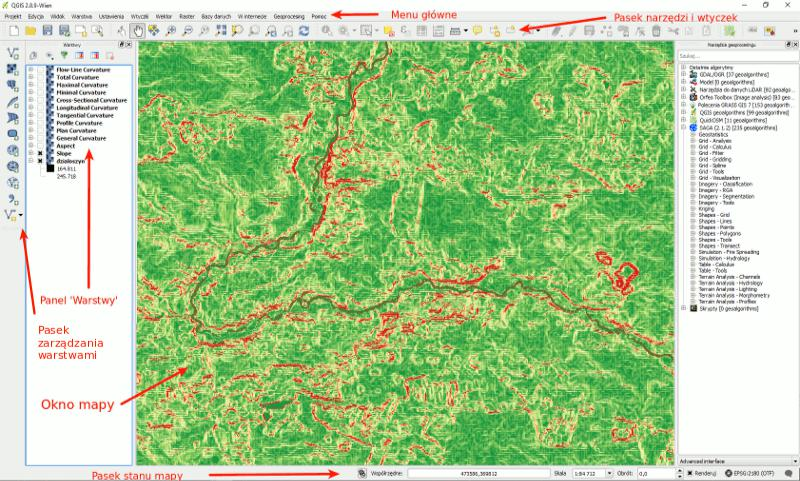
\includegraphics[width=17cm,height=10.216cm]{001-interfejs.jpg}
\caption{Główne okno programu}
\end{figure}
\end{center}
Aby dalsza praca z programem przebiegała bezproblemowo, warto zapoznać się z ogólnym układem interfejsu użytkownika QGIS. Na najważniejsze jego elementy składają się:

\begin{itemize}
\item menu główne
\item pasek narzędzi i wtyczek
\item okno mapy
\item dokowalne panele
\item pasek stanu mapy
\item pasek zarządzania warstwami
\end{itemize}

\begin{center}
\begin{figure}
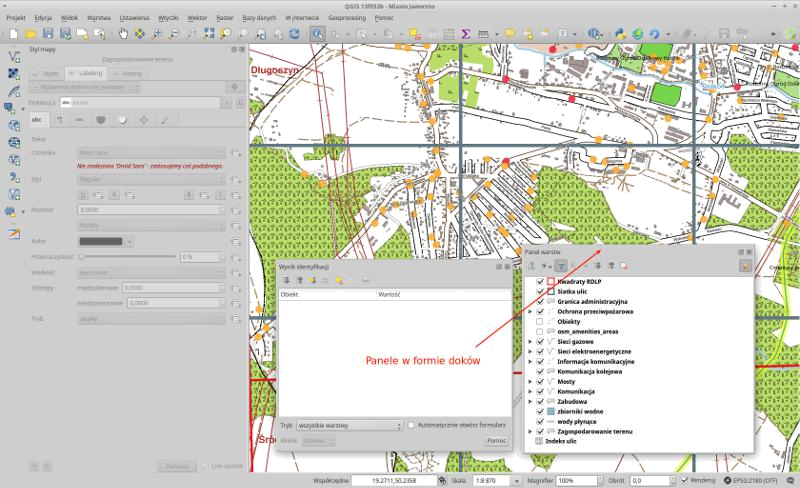
\includegraphics[width=13.219cm,height=8.061cm]{001-panele.png}
\caption{Panel w formie doków}
\end{figure}
\end{center}
Na kolejnych ilustracjach można zobaczyć przykłady konfiguracji okna programu. Panel Styl warstwy dostępny jest dopiero od wersji 2.16.
\begin{center}
\begin{figure}
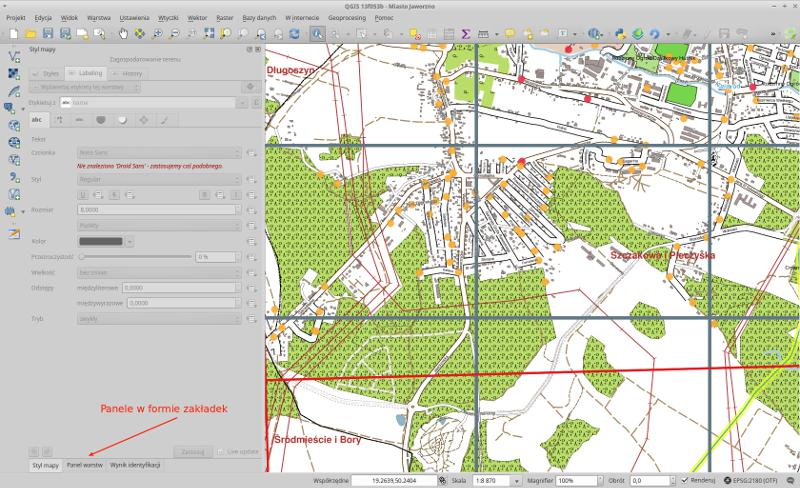
\includegraphics[width=12.961cm,height=7.426cm]{001-zakladki.jpg}
\caption{Panel w formie zakładek}
\end{figure}
\end{center}
Stopniowo rozwijane możliwości programu powodują dodawanie stale nowych funkcjonalności do interefejsu użytkownika. Przykładem są tu \textbf{Obrót} który pojawił się od wersji 2.6 oraz \textbf{Magnifier} od wersji 2.14. Służą one do zmiany obrazu mapy, bez zmiany skali wizualizacji, czy dostosowania orientacji mapy do interesującego nas obszaru.

\subsection{Ustawienia środowiska pracy}
Przed rozpoczęciem dalszej pracy omówimy konfigurację środowiska pracy, instalację najpraktyczniejszych modułów i wtyczek do QGIS. Pozwoli na to na wydajniejszą i pozbawioną niespodziewanych problemów dalszą pracę.

Rozpoczniemy od wybrania z menu głównego programu Ustawienia -{\textgreater} Opcje. Pojawi się nam okno opcji konfiguracyjnych programu. Przejdźmy do zakładki System. 

\begin{center}
\begin{figure}
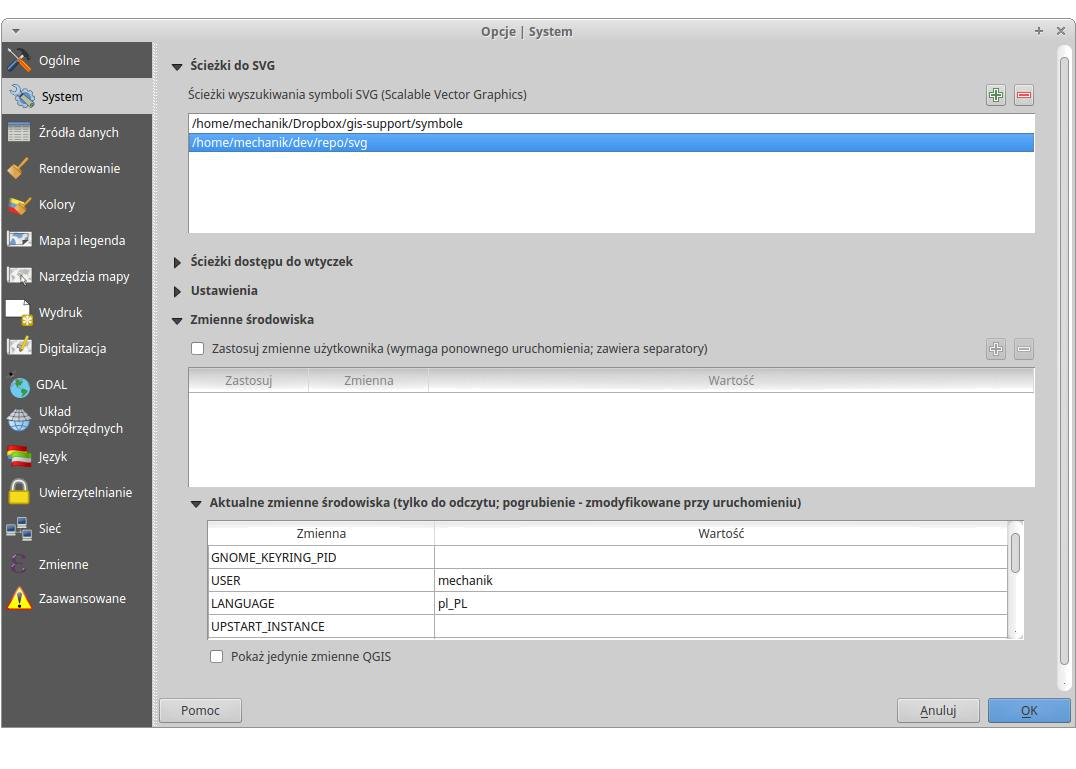
\includegraphics[width=13.014cm,height=9.282cm]{002-zakladka-system.png}
\caption{Ustawienia - Zakładka System}
\end{figure}
\end{center}
W pierwszym polu od góry \textbf{Ścieżki do SVG }wskazujemy ścieżkę dostępu do katalogu w którym znajdują się nasze repozytoria symboli kartograficznych. Szczególnie przy redakcji kartograficznej, oraz współdzieleniu projektów jest to wygodne rozwiązanie, pozwalające na stosowanie relatywnych odwołań do plików. Następną istotną zakładką jest \textbf{Renderowanie}.

\begin{center}
\begin{figure}
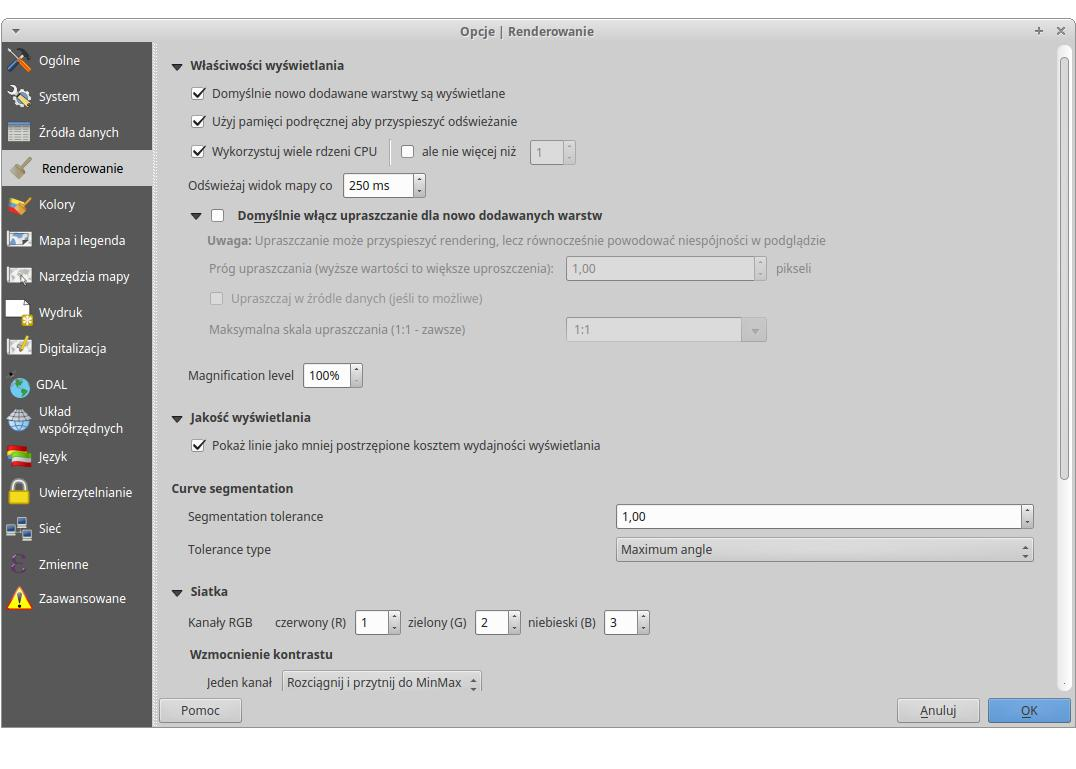
\includegraphics[width=13.014cm,height=9.275cm]{002-zakladka-renderowanie.jpg}
\caption{Ustawienia - Zakładka Renderowanie}
\end{figure}
\end{center}
W tej zakładce możemy dostosować ustawienia związane z prędkością i jakością renderowania podglądu mapy w oknie głównym. W grupie Właściwości wyświetlania szczególnie istotnym jest pozycja \textbf{Wykorzystaj wiele} \textbf{rdzeni CPU.} Grupa Domyślnie włącz upraszczanie dla nowo dodawanych warstw powinna pozostać wyłączona, jeśli chcemy pracować z danymi topologicznymi, albo stosować przyciąganie (snapping).

\begin{center}
\begin{figure}
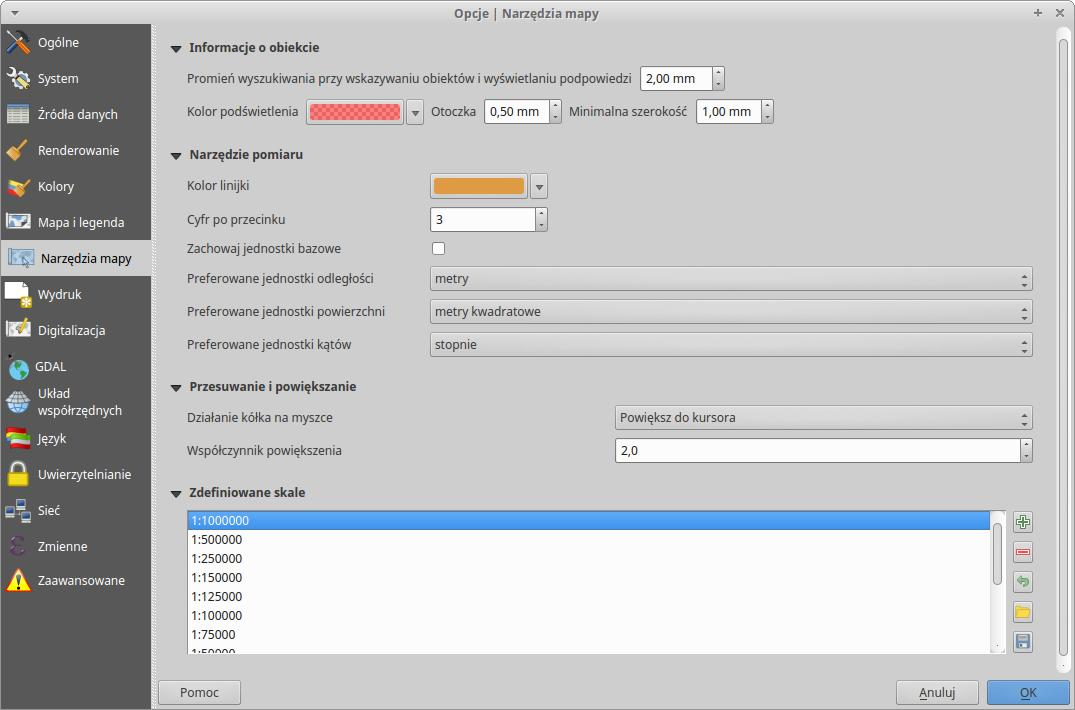
\includegraphics[width=17cm,height=8.562cm]{002-zakladka-narzedzia.jpg}
\caption{Ustawienia - Zakładka Narzędzia Mapy}
\end{figure}
\end{center}
W zakładce Kolory możemy zarządzać dostępnymi paletami barwnymi, np. przygotowując wcześniej zdefiniowany zestaw kolorów dla mapy/projektu. W zakładce tej możemy również zaimportować pliki palet barwnych, zgodnych z formatem Gimp Palette.

W zakładce Narzędzia mapy znajdują się pola dla zdefiniowania wyglądu obiektów zaznaczonych, linijki pomiarowej, jednostek miary. W grupie Zdefiniowane skale możemy wprowadzić skale mapy, które mają być stosowane np. przy tworzeniu atlasu.


\begin{center}
\begin{figure}
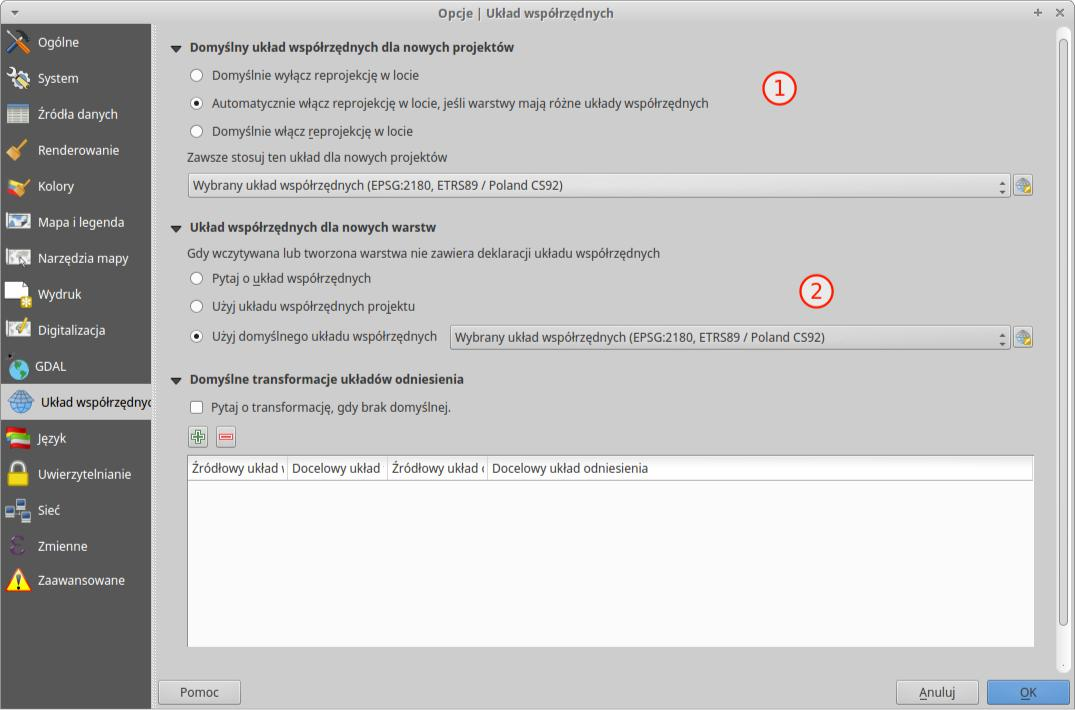
\includegraphics[width=16.997cm,height=11.19cm]{002-zakladka-uklad.jpg}
\caption{Ustawienia - Zakładka Układ Współrzędnych}
\end{figure}
\end{center}
Zakładka Układ współrzędnych jest bardzo istotna dla komfortu pracy z zbiorami danych. W grupie Domyślny układ współrzędnych dla nowych projektów warto ustawić opcję oznaczoną cyfrą 1 (\textit{Automatycznie włącz reprojekcję w l} \textit{współrzędnych}),oraz wybrać listy (lub ikonką globusa po prawej, jeśli na liście nie ma) preferowany przez nas układ i odwzorowanie. Na ilustracji widać wybór układu 1992. Cyfrą 2 w grupie Układ współrzędnych dla nowych warstw oznaczona jest pozycja, którą warto ustawić, gdy często mamy do czynienia z zbiorami danych stworzonymi uprzednio w pakiecie ArcGIS, który pozwala na zapisanie Shapefile bez definicji układu. Tu również możemy wskazać domyślny układ.

\subsection{Moduły}
Aby w pełni wykorzystać możliwości jakie daje współczesne środowisko pracy GIS, szczególnie w wersji open-source warto skorzystać z dodatkowych modułów. Szczególnie praktyczną jest integracja z SAGA GIS, oraz GRASS.

Jeśli korzystasz z systemu operacyjnego Windows, skorzystaj z wspomnianego wcześniej instalatora OSGeo4W i wybierz pakiety SAGA, GRASS.

Dla systemów Unix'owych, konieczna jest instalacja z pakietów, np. dla Ubuntu/Debiana:


sudo add-apt-repository ppa:johanvdw/saga-gis 
\\sudo apt-get update
\\sudo apt-get install saga qgis-plugin-grass grass-core


Następnie pobierz pakiet LASTools ze strony producenta: \url{https://rapidlasso.com/lastools/} i rozpakuj do katalogu, zapisując ścieżkę dostępu.

Istnieje również możliwość skorzystania z pakietu Fusion/LDV opracowanego przez Departament Rolnictwa USA: \url{http://forsys.cfr.washington.edu/fusion/fusionlatest.html} Gdy mamy już przygotowane pakiety, wybieramy z menu QGIS Geoprocessing -{\textgreater} Opcje i z zakładki Narzędzia do danych LiDAR wybieramy \textbf{Aktywuj }a następnie wprowadzamy ścieżki dostępu do wcześniej zainstalowanego Fusion/LDV i LASTools (oba pakiety są opcjonalne i niewymagane do pracy).



\begin{center}
\begin{figure}
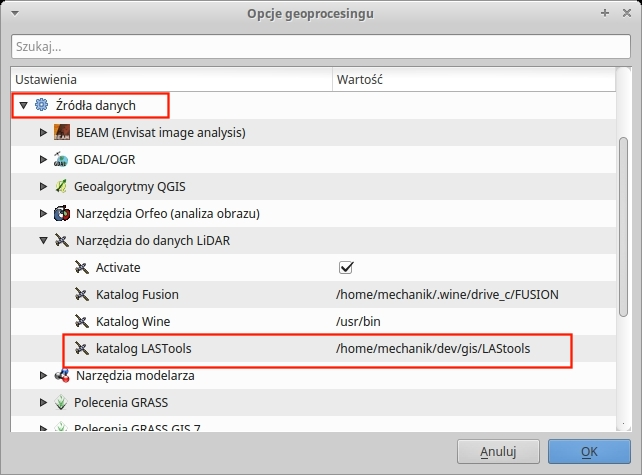
\includegraphics[width=16.838cm,height=12.457cm]{002-lidar.jpg}
\caption{Konfiguracja modułów LiDAR w Ubuntu}
\end{figure} 
\end{center}
Następnie w zakładce SAGA również korzystamy z pola \textbf{Włącz}. W Ubuntu dodatkowo wypełniamy ścieżkę dostępu do pliku wykonywalnego pakietu Wine (wymagany dla poprawnej pracy LASTools).

Jeśli ustawione przez nas parametry są już poprawne zatwierdzamy klawiszem \textbf{OK},, następuje sprawdzenie konfiguracji i możemy przystąpić do dalszej pracy.

Inne dostępne moduły:

\begin{itemize}
\item TauDEM - \url{http://hydrology.usu.edu/taudem/taudem5/index.html}
\item Orfeo Toolbox - \url{https://www.orfeo-toolbox.org/}
\item R toolbox - \url{https://www.r-project.org/}
\item BEAM and SNAP (Sentinel-1, Sentinel-2, Envisat) - \url{http://step.esa.int}
\end{itemize}
\subsection{Modelarz graficzny}
Rozszerzenie Processing udostępnia również tzw. modelarz graficzny. Pozwala on w graficznym interfejsie użytkownika stworzyć łańcuch narzędzi, oraz zbiorów danych,i wskazać kolejność ich przetwarzania. Istnieje również możliwość ich zapisania do ponownego wykorzystania. Szczególnie przydatne jest to przy przetwarzaniu danych pochodzących ze skanowania laserowego czy interpolacji danych wektorowych do postaci rastrowej.



\begin{center}
\begin{figure}
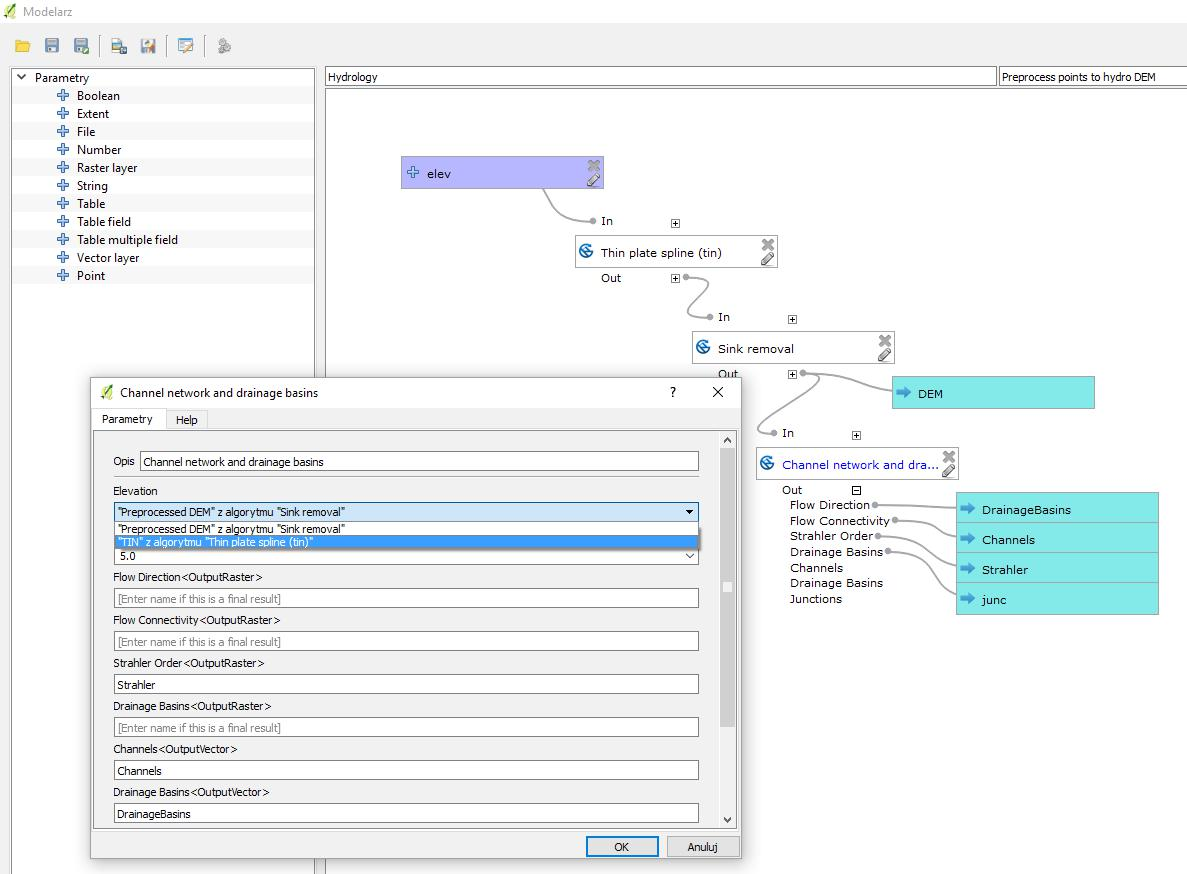
\includegraphics[width=12.562cm,height=9.229cm]{002-modelarz.jpg}
\caption{Modelarz graficzny}
\end{figure}
\end{center}
\subsection[Wtyczki]{Wtyczki}
QGIS wykorzystuje w swoim działaniu modułową budowę, opartą o biblioteki działające w tle takie jak GDAL/OGR, python-qgis, rdzeń programu realizujący zarządzanie procesami, oraz rozszerzające funkcjonalność wtyczki (plugins), dostępne w QGIS Plugins Repository.

\ \ Zawiera ono setki wtyczek, niektóre z nich oznaczone jako eksperymentalne - pamiętaj, że mogą one nie działać tak jakbyś chciał. Aby móc skorzystać z tej funkcjonalności, konieczny jest zainstalowany interpreter języka Python (dla Windows najlepiej skorzystaj z instalatora OSGeo4W). Następnie w QGIS wybieramy opcję menu Wtyczki -{\textgreater} Zarządzaj wtyczkami



\begin{center}
\begin{figure}
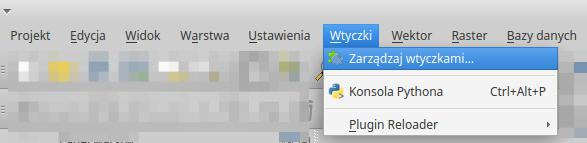
\includegraphics[width=13cm,height=3.14cm]{002-wtyczki-zarzadzanie.jpg}
\caption{Zarządzanie wtyczkami}
\end{figure}
\end{center}


\begin{center}
\begin{figure}
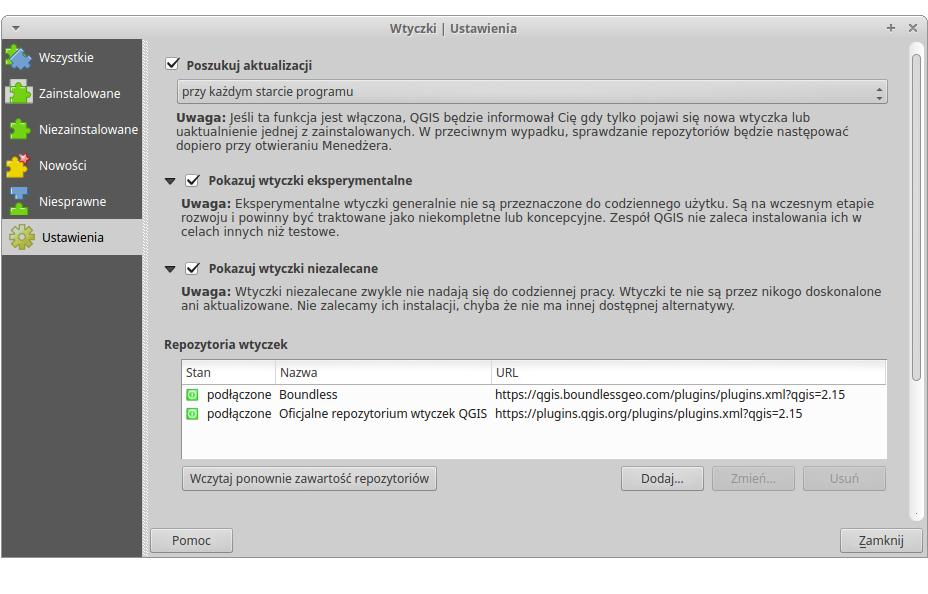
\includegraphics[width=13.014cm,height=8.311cm]{002-wtyczki-repo.jpg}
\caption{Repozytorium wtyczek}
\end{figure}
\end{center}
Po otwarciu okna wybieramy zakładkę Ustawienia.

Przy jej pomocy możemy włączyć dostęp do wtyczek eksperymentalnych, lub niezalecanych, a także samodzielnie zdefiniować zewnętrzne repozytoria wtyczek (plugins) QGIS.

W kolejnym etapie przechodzimy do zakładki ``Wszystkie'' gdzie możemy rozpocząć proces dodawania interesujących nas wtyczek. Niektóre z nich są bezpośrednio dostępne do włączenia (np. Georeferencer GDAL, Glob, czy Rastrowe Analizy Terenu). Inne należy zainstalować wpisując ich nazwę w oknie wyszukiwania lub wybierając z listy, a następnie korzystając z przycisku ``Zainstaluj wtyczkę'' oznaczonego cyfrą jeden na poniższej ilustracji.

W naszym przypadku zainstalujemy następujące wtyczki:

\begin{center}
\begin{itemize}
\item QuickOSM
\item go2StreetView
\item eVis
\item TableManager
\item QuickMapServices
\item TimeManager
\item qgis2web
\item Resource Sharing
\end{itemize}
\end{center}
Upewnimy się również czy włączony został Georeferencer GDAL.

\begin{center}
\begin{figure}
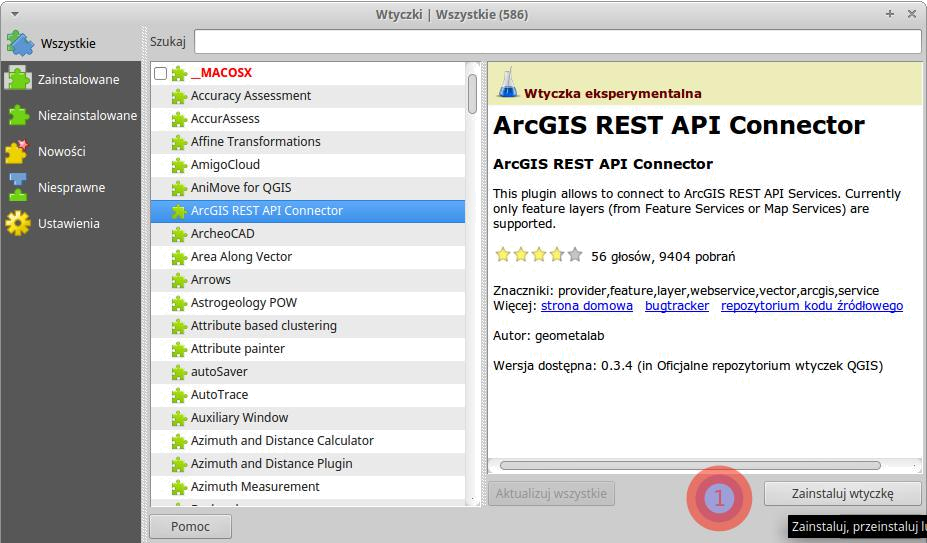
\includegraphics[width=13cm,height=7.592cm]{002-wtyczki-instalacja.png}
\caption{Instalacja wtyczek}
\end{figure}
\end{center}
\section{Projekt}
W środowisku QGIS \textbf{Projekt }jest zbiorem warstw, stylizacji, arkuszy kompozera wydruków, a także reguł, zapytań bazodanowych zapisanych do ponownego użycia. Dlatego tak istotnym jest zrozumienie i prawidłowe wykorzystanie jego możliwości. W tym bloku omówimy konfigurację projektu, tworzenie metadanych, definiowanie układów współrzędnych, oraz projektowe ustawienia serwera usług sieciowych.
Po uruchomieniu QGIS w wersji LTR środowisko przygotowane jest do pracy z nowym projektem, zaś od wersji 2.14 w oknie mapy wyświetlana jest lista ostatnio otwartych projektów, do szybkiego otwarcia. Przy tym otwarcie dowolnej warstwy danych przywraca okno mapy i można rozpocząć pracę.

Wszystkie operacje związane z projektem realizowane są przy pomocy menu Projekt, znajdującego się na pierwszej pozycji menu QGIS.

\subsection{Opis i metadane}
Większość pracy związanej z konfiguracją projektu można zrealizować poprzez wywołanie \textbf{Właściwości projektu} z menu Projekt - Właściwości projektu. Można też skorzystać z skrótu klawiszowego Ctrl+Shift+P.

Po otwarciu okna właściwości projektu zobaczymy podobny układ treści z zakładkami po lewej stronie. W pierwszej zakładce \textbf{Ogólne }najpraktyczniejsze pozycje to, oznaczone cyfrą jeden pole \textbf{Tytuł} \textbf{projektu, }w którym wprowadzamy ogólną\textbf{nazwę projektu}, która będzie wyświetlana w przyszłości na liście ostatnich projektów, w oknie głównym programu, etc.

Pod cyfrą dwa kryje się opcja \textbf{Zapisz ścieżki} która może być bardzo przydatna przy przenoszeniu projektu pomiędzy stanowiskami roboczymi, ustawienie \textit{Względne}powoduje że zapisywane są lokalizacje plików warstw, oraz symboli względem pliku\textit{projektu}.

Pod pozycją trzy możemy zdefiniować \textbf{Skale projektu}



\begin{center}
\begin{figure}
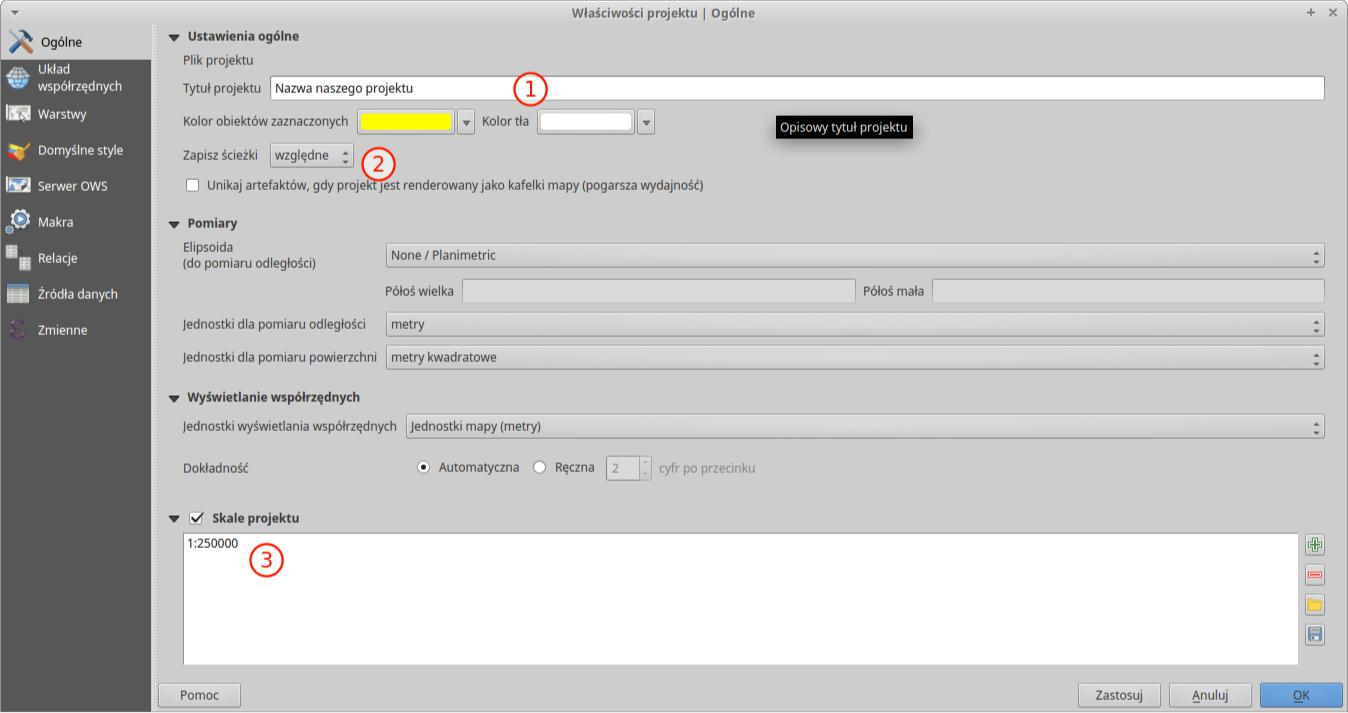
\includegraphics[width=13cm,height=6.858cm]{002-projekt.png}
\caption{Właściwości projektu}
\end{figure}
\end{center}


\begin{center}
\begin{figure}
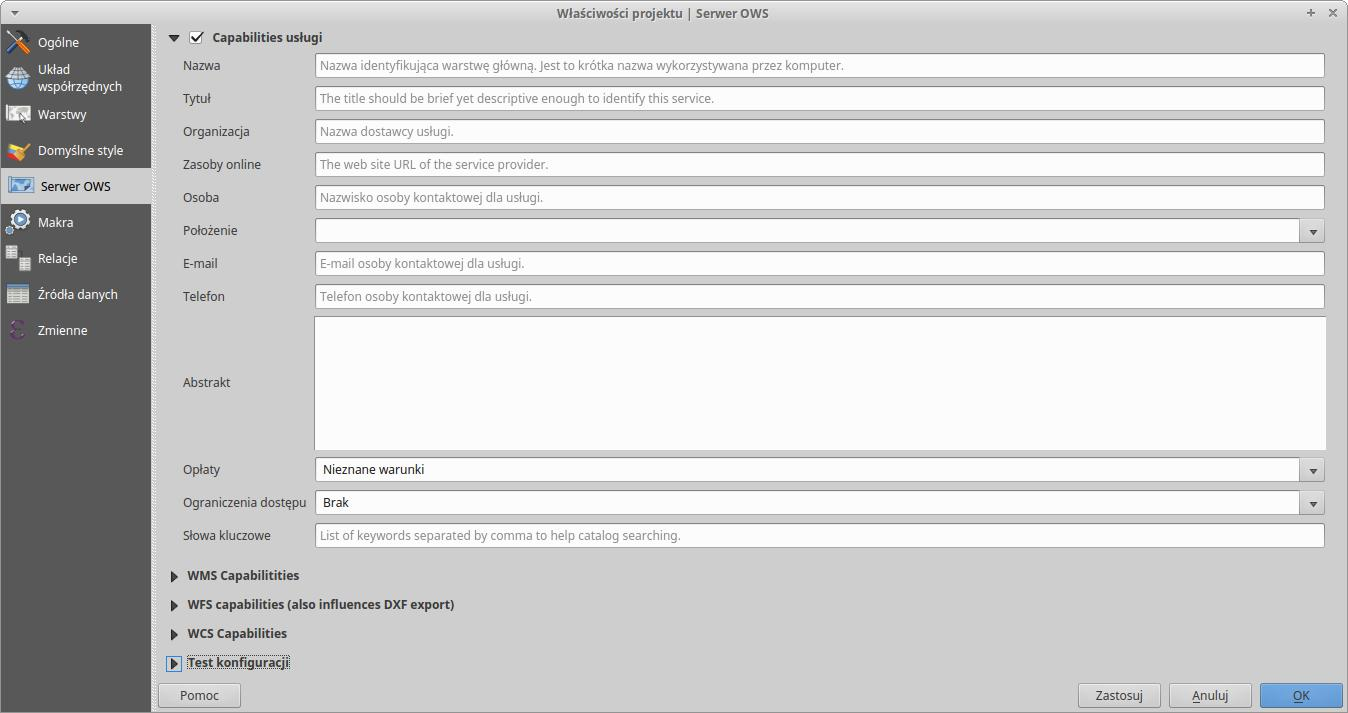
\includegraphics[width=13cm,height=6.862cm]{002-projekt-ows.jpg}
\caption{Metadane i ustawienia serwera OWS}
\end{figure}
\end{center}
W przypadku skorzystania z zakładki \textbf{Serwer OWS możemy }zdefiniować komplet metadanych publikowanych przy pomocy usług sieciowych WMS, WFS, WCS. W polach WMS Capabilities, WFS Capabilities możemy wybrać sposób publikowania warstw danych (dostępność układów współrzędnych, zasięg rozgłaszany, etc.)

\subsection{CRS}
W zakładce Układ współrzędnych możemy wybrać z listy istniejący układ współrzędnych, wyszukując go w oknie Filtr po nazwie, cechach charakterystycznych, lub kodzie EPSG.

W przypadku popularnych odwzorowań i układów współrzędnych (np. WGS84, UTM) jest to bardzo proste i wygodne rozwiązanie. Niestety w przypadku map archiwalnych, czy dla nietypowych obszarów, system odniesień przestrzennych (CRS) może nie być zdefiniowany w bazie kodów EPSG. Wtedy koniecznym staje się jego samodzielne utworzenie. Aby to uczynić z wybieramy z menu programu Ustawienia -{\textgreater} Układ współrzędnych użytkownika. Po otwarciu okna z prawej strony u góry widoczny jest przycisk z zielonym symbolem +. Na ilustracji oznaczony został cyfrą jeden.



\begin{center}
\begin{figure}
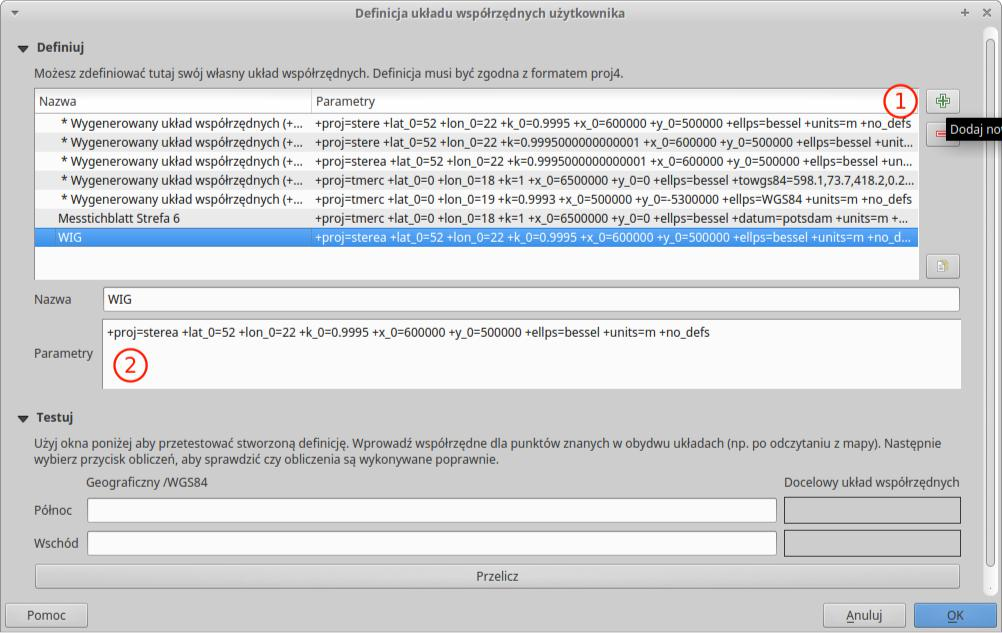
\includegraphics[width=13.998cm,height=8.809cm]{002-crs.jpg}
\caption{Tworzenie definicji CRS}
\end{figure}
\end{center}
Po kliknięciu w ten przycisk w pole nazwa wpisujemy własną nazwę układu, zaś w pole parametry informację zgodną z definicją dla biblioteki PROJ.4. Każdy z parametrów rozpoczyna się symbolem +, z wartością za znakiem =. Symbol +k\_0 oznacza zmniejszenie skali na południku osiowym.

Przykładowa, widoczna na ilustracji definicja układu odpowiada parametrom układu współrzędnych Wojskowego Instytutu Geograficznego, za wyjątkiem definicji odwzorowania (odwzorowanie Rousillhe'a nie jest obsługiwane w tym miejscu programu), konieczne jest więc skorzystanie z odwzorowania stereograficznego. W przykładzie wskazana jest również elipsoida Bessela. Po zakończeniu wprowadzania, mamy możliwość przetestowania poprawności transformacji dla znanych współrzędnych. Na koniec wybieramy opcję \textbf{OK}.Jeśli definicja układu jest poprawna, okno zostanie zamknięte i CRS będzie dostępny do wykorzystania w pozostałych miejscach programu.

\section{Praca z warstwami danych}
\ \ W kolejnym bloku zajęć poruszymy tematykę prostych operacji otwierania, zapisywania, czy transformacji układu zbiorów.

\subsection{Otwieranie warstwy}

\begin{center}
\begin{figure}
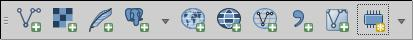
\includegraphics[width=10.929cm,height=1.058cm]{002-pasek-warstwy.jpg}
\caption{Pasek zarządzania warstwami}
\end{figure}
\end{center}
Z lewej strony okna programu standardowo widoczny jest pionowy pasek zarządzania warstwami. Na ilustracji powyżej, pasek ten został odpięty z swojego miejsca i obrócony do orientacji poziomej. Operacja ta została wykonana dla zwiększenia czytelności i nie wpływa na funkcjonalność tego narzędzia.

W tym rozdziale zaprezentujemy kolejno sposób otwierania zbiorów danych dostępnych w QGIS. Kolejność ta będzie zgodna z widocznymi ikonkami.



\begin{center}
\begin{figure}
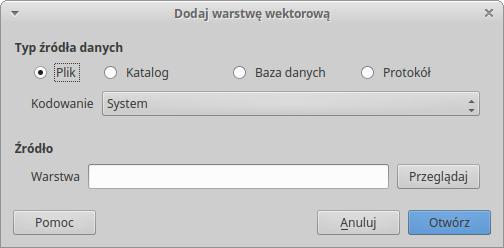
\includegraphics[width=11.698cm,height=5.75cm]{002-dodaj-wektor.jpg}
\caption{Dodawanie warstwy wektorowej}
\end{figure}
\end{center}
W przypadku warstwy wektorowej otworzy się okno z niewielką ilością opcji.Dla zbiorów w formatach Shapefile, GeoJSON, DXF, czy innych plikowych powinniśmy skorzystać z Typ źródła danych -{\textgreater} Plik.

Dla geobazy \textit{.gdb (ArcGIS)} właściwą opcją jest typ\textit{\textbf{Katalog}}.



\begin{center}
\begin{figure}
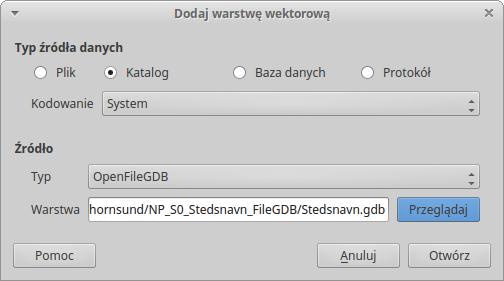
\includegraphics[width=13.335cm,height=7.437cm]{002-dodaj-ogdb.png}
\caption{Dodawanie warstwy wektorowej - geobaza}
\end{figure}
\end{center}
Konieczne jednak w tym momencie jest wskazanie również podtypu źródła danych. Dla geobazy wybieramy OpenFileGDB.

W przypadku formatów danych które pozwalają na przechowywanie w jednym zbiorze wielu tabel, lub wielu typów geometrii, takich jak **GeoJSON, GPX** czy właśnie geobaza, zobaczymy kolejne okno, wyboru warstw do dodania. Każda zaznaczona warstwa zostanie zaczytana do wykorzystania w programie.



\begin{center}
\begin{figure}
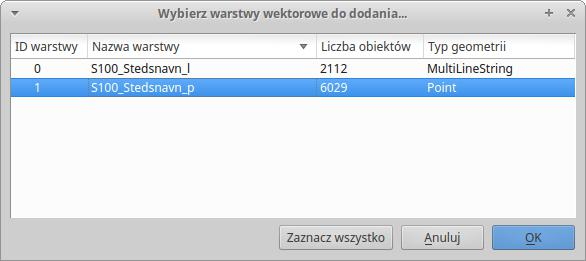
\includegraphics[width=13cm,height=5.779cm]{002-typ-geometrii.jpg}
\caption{Selekcja warstw zbioru z wieloma typami geometrii}
\end{figure}
\end{center}
Kolejnym jest format danych rastrowych. Tutaj operacja jest dużo prostsza, każdy z dostepnych formatów obsługiwany jest identycznie, poprzez okno wyboru pliku.

W przypadku baz danych (Spatialite, PostGIS, Oracle Spatial, MSSQL) okno otwarcia jest podobne, różni się wyłącznie opcjami specyficznymi dla wybranej bazy.

\begin{center}
\begin{figure}
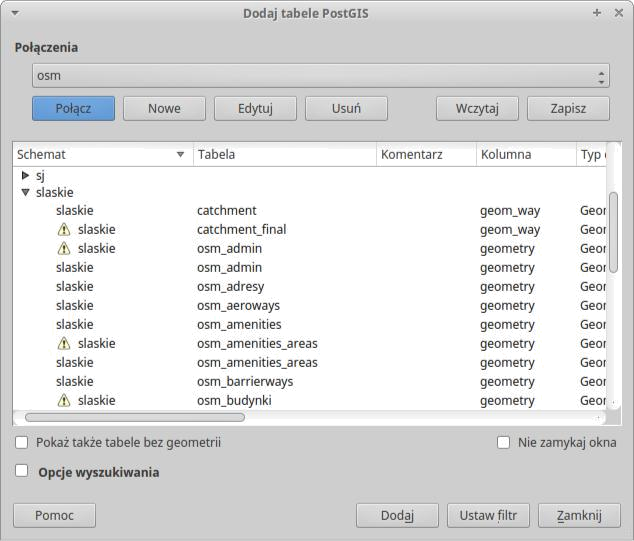
\includegraphics[width=13cm,height=11.077cm]{002-dodaj-postgis.png}
\caption{Dodawanie warstw PostGIS}
\end{figure}
\end{center}

\begin{center}
\begin{figure}
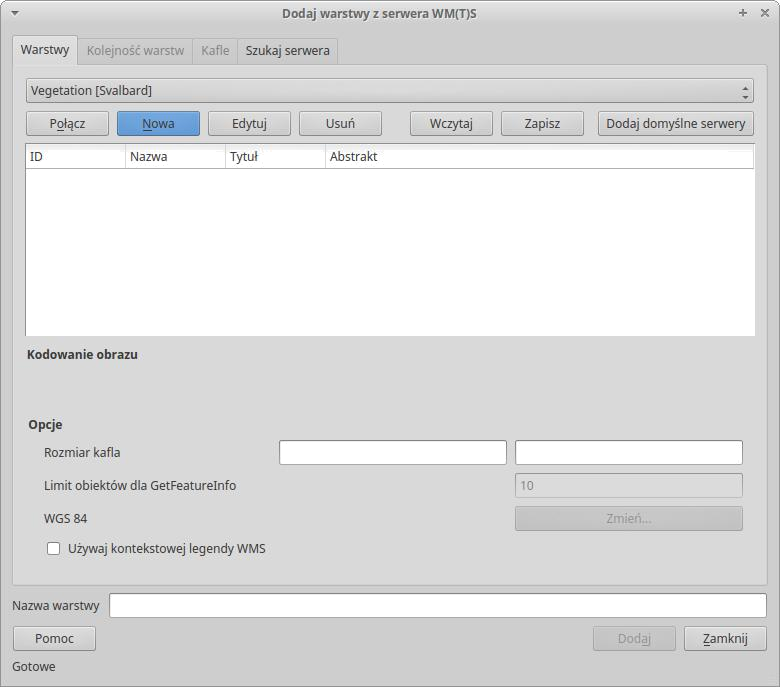
\includegraphics[width=13cm,height=11.43cm]{002-dodaj-wms.png}
\caption{Usługi sieciowe WMS}
\end{figure}
\end{center}

Kolejne ikony odpowiadają za otwieranie usług sieciowych WMS, WFS, WCS. Otwarcie takiej warstwy omówimy na przykładzie WMS Mapy topograficznej w Geoporrtalu krajowym.

Po wybraniu \textbf{Dodaj warstwę WMS/WMTS} naszym oczom ukazuje się okno jak na ilustracji poniżej. Wybieramy przycisk Nowy.

\begin{center}
\begin{figure}
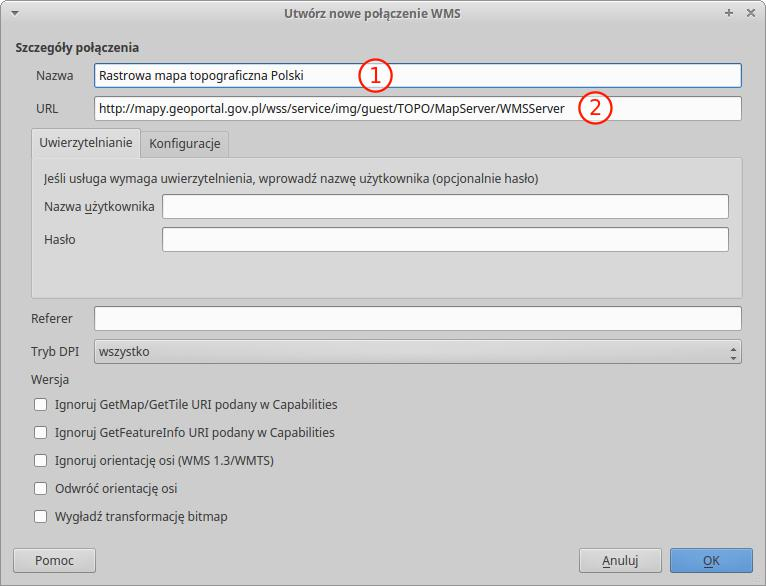
\includegraphics[width=13cm,height=9.931cm]{002-tworzenie-wms.jpg}
\caption{Tworzenie nowego wpisu dla usługi WMS}
\end{figure}
\end{center}
Po wczytaniu z serwera listy warstw, możemy dokonać wyborów warstw, formatu kodowania obrazu (jeśli chcesz uzyskać przezroczystość warstwy WMS, np. w celu wyświetlenia wielu różnych serwisów, skorzystaj z ustawień *PNG/PNG8*). Poniżej istnieje możliwość zmiany układu współrzędnych (a przez to i odwzorowania), z której warto skorzystać, estetyka układu WGS84 odstaje od naszych przyzwyczajeń. Na koniec wybieramy przycisk Dodaj, a po nim Zamknij. Wczytana warstwa WMS pojawi się w oknie mapy, oraz na liście warstw.
W podobny sposób można dodać warstw danych z usług Web Feature Service, oraz Web Coverage Service.

\subsection{Zapisz jako}
Gdy zachodzi konieczność zapisania do nowego zbioru danych które utworzyliśmy, dokonaliśmy ich selekcji, lub chcielibyśmy wykonać transformację układu współrzędnych, powinniśmy skorzystać z funkcji **Zapisz jako** dostępnej z menu kontekstowego warstwy - wywołujemy je prawym klawiszem myszy w obrębie listy warstw.



\begin{center}
\begin{figure}
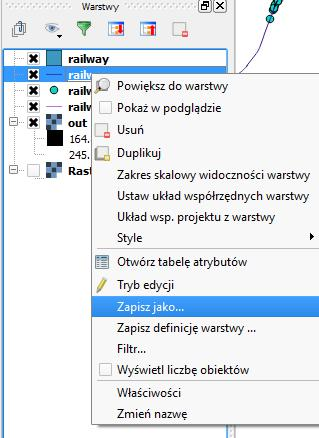
\includegraphics[width=8.435cm,height=11.557cm]{002-menu-kontekstowe.jpg}
\caption{Menu kontekstowe warstwy}
\end{figure}
\end{center}
W przypadku warstwy wektorowej po wprowadzeniu nazwu (np. przy użyciu przycisku **Przeglądaj**), oraz wskazaniu
docelowego układu współrzędnych, możemy wybrać również docelowe kodowanie tekstu (preferowane UTF-8), oraz jeśli tworzona wartstwa jest selekcją z innej, powinniśmy zaznaczyć opcję  Zapisz tylko wybrane . Pozostałe pozycje w oknie zależą od kontekstu formatu warstwy wektorowej i mogą pozostać domyślne, *{\textquotedbl}jeśli nie wiesz co oznaczają{\textquotedbl}*.

\begin{center}
\begin{figure}
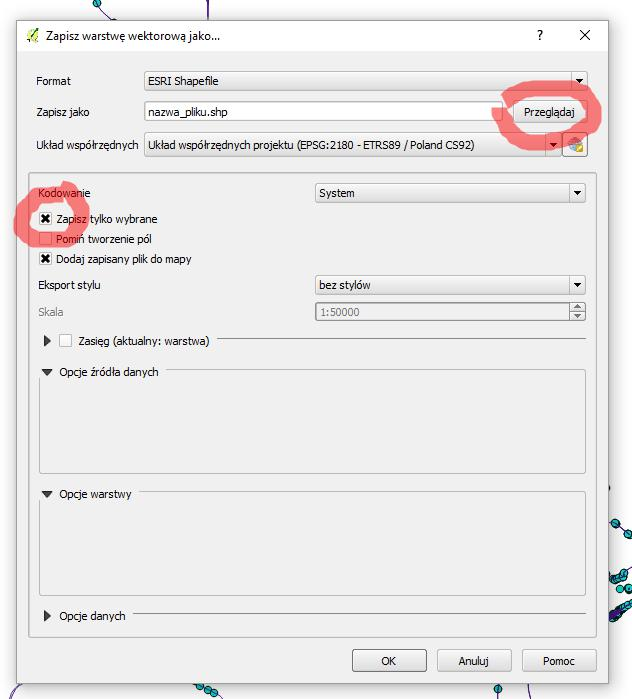
\includegraphics[width=13cm,height=14.372cm]{002-zapisz-wektor.jpg}
\caption{Okno zapisu warstwy wektorowej}
\end{figure}
\end{center}
Dla warstwy rastrowej ilośc opcji jest trochę większa. Możemy między innymi zmienić rozdzielczość warstwy wynikowej, (podaną w jednostkach CRS wybranego powyżej - uwaga przy układach geograficznych, jednostkami są stopnie). Możemy również włączyć kompresję oraz przygotować piramidy skalowe.

\begin{center}
\begin{figure}
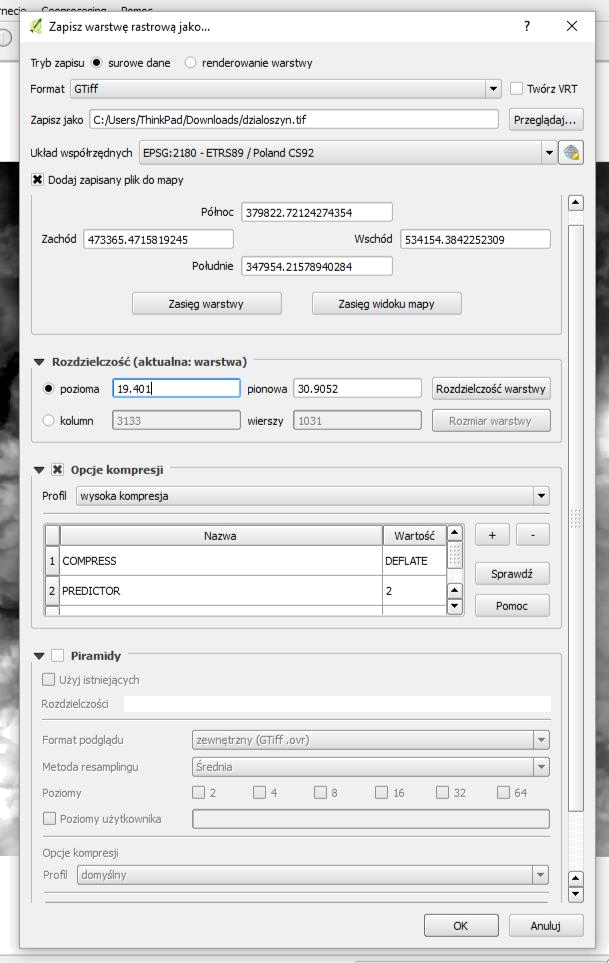
\includegraphics[width=13cm,height=20.546cm]{002-zapisz-raster.png}
\caption{Okno zapisu warstwy rastrowej}
\end{figure}
\end{center}

\subsection[Nowa warstwa]{Nowa warstwa}
W QGIS możemy utworzyć nową warstwę danych wektorowych, nie tylko poprzez
selekcję obiektów z istniejącego zbioru, ale również przy pomocy funkcji \textbf{Nowa warstwa} \textbf{Shapefile},czy \textbf{Nowa warstwa}.\textbf{ tymczasowa}

Dla warstwy typu ESRI Shapefile należy uzupełnić po kolei parametry warstwy takie jak typ geometrii, kodowanie, CRS, następnie dodać atrybuty (kolumny) do tabeli. Każdorazowo musimy pamiętać o ograniczeniach formatu Shapefile, tj. nazwa atrybutu nie może być dłuższa niż 8 znaków. Po zatwierdzeniu klawiszem OK zostaniemy zapytani o nazwę pliku dla zbioru danych.

\begin{center}
\begin{figure}
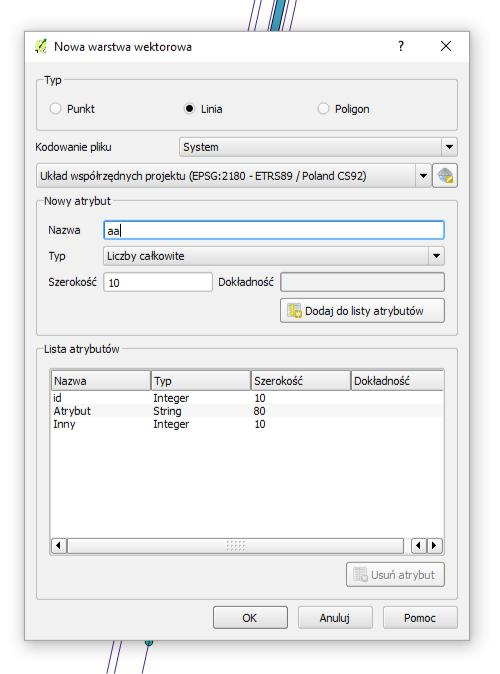
\includegraphics[width=11.599cm,height=15.579cm]{002-nowy-wektor.jpg}
\caption{Tworzenie nowej warstwy Shapefile}
\end{figure}
\end{center}
Gdy chcemy obejść ograniczenia formatu Shapefile, QGIS pozwala nam na skorzystanie z warstwy \textit{tymczasowej}. W jej przypadku definiujemy wyłącznie typ geometrii, oraz CRS warstwy. Nie są dokonywane żadne zmiany na dysku, musimy pamiętać o samodzielnym zapisaniu po zakończeniu pracy z warstwą. Aby wykonać więcej  operacji związanych z tworzeniem zbioru danych wetorowych warto skorzystać z wtyczki „Table Manager”.

\chapter{Warstwy wektorowe i CSV}
Kolejny blok zajęć wymaga trochę przypomnienia podstawowych pojęć z zakresu grafiki i geometrii. W praktyce GIS przyjęło się rozdzielać typy warstw na wektorowe i rastrowe.

W praktyce GIS przyjęło się wszystkie zbiory danych, w których geometria jest opisana ciągiem współrzędnych kartezjańskich lub kątowych, nazywać \textbf{wektorowymi}.Dziedzictwo pierwszych systemów GIS, oraz formatu Shapefile powoduje że wciąż operujemy również pojęciem \textbf{typu geometrii}.Oto przykłady:

\section{Operacje przestrzenne}
QGIS w operacjach przestrzennych opiera się na zewnętrznych modułach i bibliotekach takich jak GEOS, MMGIS i inne. Większość narzędzi do operacji zależności przestrzennych znajduje się w menu Wektor -{\textgreater} Narzędzia geoprocesingu.

\begin{center}
\begin{figure}
\caption{Narzędzia geoprocessingu}
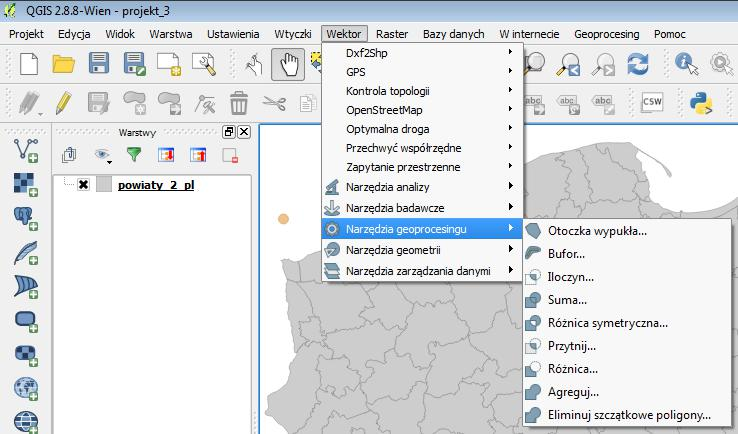
\includegraphics[width=9.37cm,height=5.514cm]{003-geoprocessing.jpg}
\end{figure}
\end{center}

\begin{itemize}
\item otoczka wypukła - tworzy warstwę z najmniejszym poligonem (otoczką) zawierającym całą warstwę lub poligonami okalającymi poszczególne jej obiekty, opierając się na polu z unikalną wartością
\item bufor - tworzy strefę buforową o zadanej szerokości wokół obiektów lub na podstawie wartości atrybutu; możliwa jest agregacja buforów w jeden obiekt;
\begin{center}
\begin{figure}
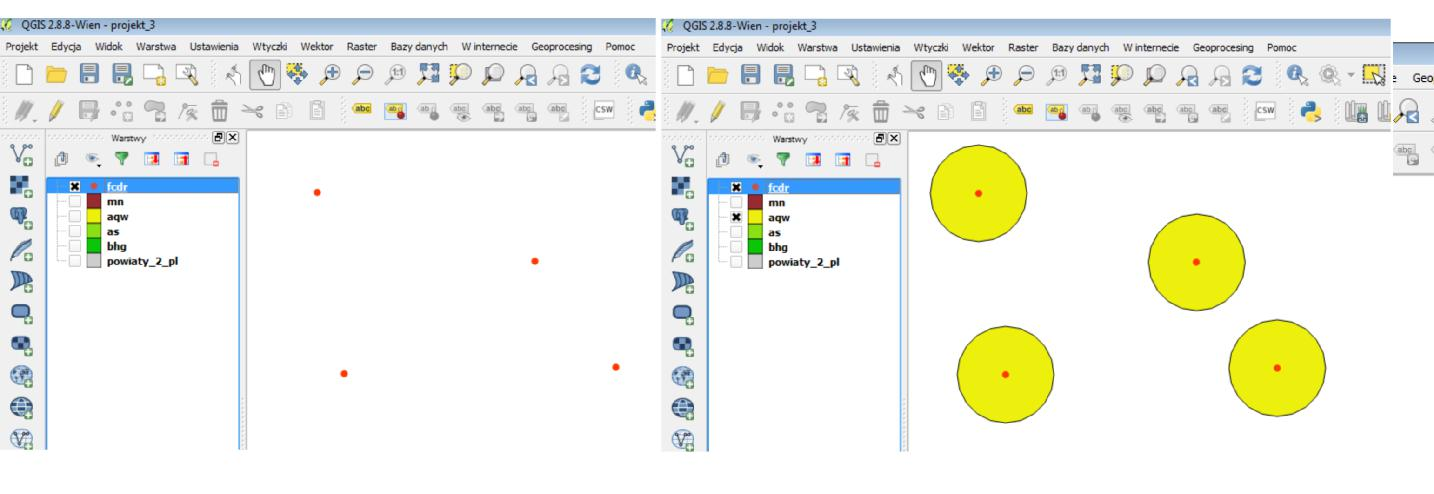
\includegraphics[width=16.859cm,height=5.803cm]{003-bufor.jpg}
\caption{Wynik operacji Bufor}
\end{figure}
\end{center}
\item iloczyn (intersect) - tworzy nowe obiekty będące częściami wspólnymi obiektów z dwóch warstw; do tabeli zostają dołączone atrybuty obu warstw;
\begin{center}
\begin{figure}
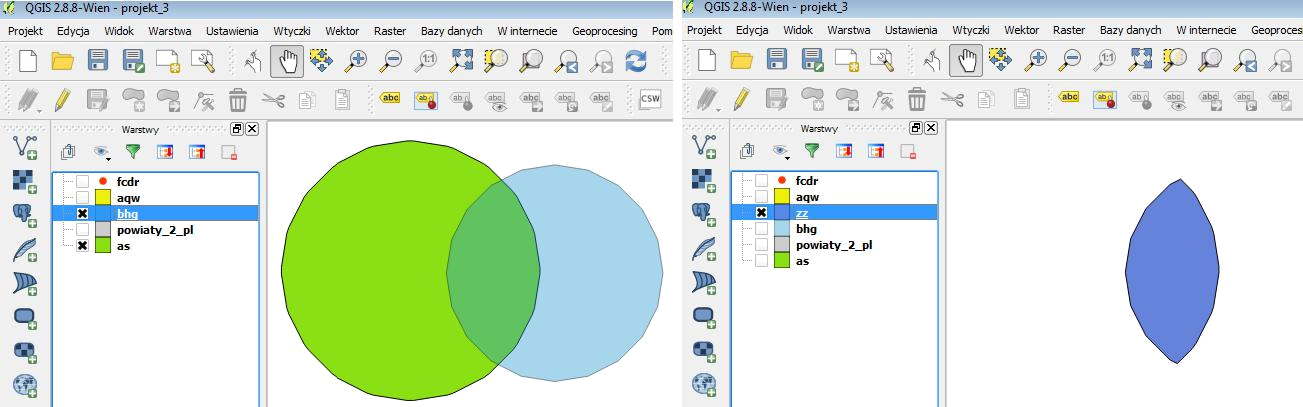
\includegraphics[width=16.365cm,height=5.112cm]{003-iloczyn.png}
\caption{Wynik operacji Iloczyn}
\end{figure}
\end{center}
\item suma (union) - tworzy nowe obiekty będące częściami wspólnymi obiektów z dwóch warstw oraz obiektów, które się nie nakładają; do tabeli zostają dołączone atrybuty obu warstw;
\begin{center}
\begin{figure}
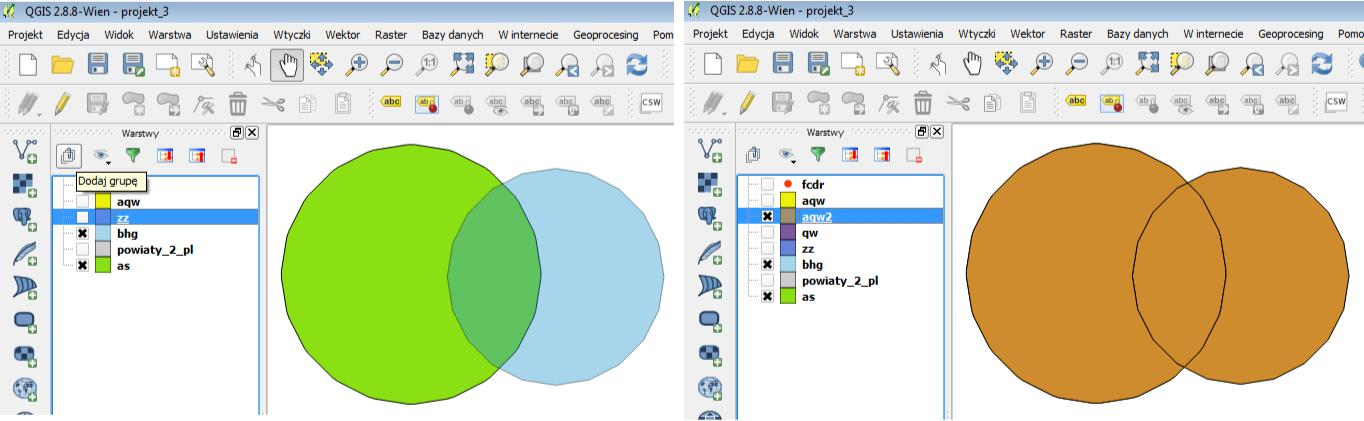
\includegraphics[width=16.365cm,height=5.048cm]{003-suma.jpg}
\caption{Wynik operacji Suma}
\end{figure}
\end{center}
\item różnica symetryczna - tworzy nowe obiekty, z obiektów dwóch warstw, które się nie pokrywają; do tabeli zostają dołączone atrybuty obu warstw;
\begin{center}
\begin{figure}
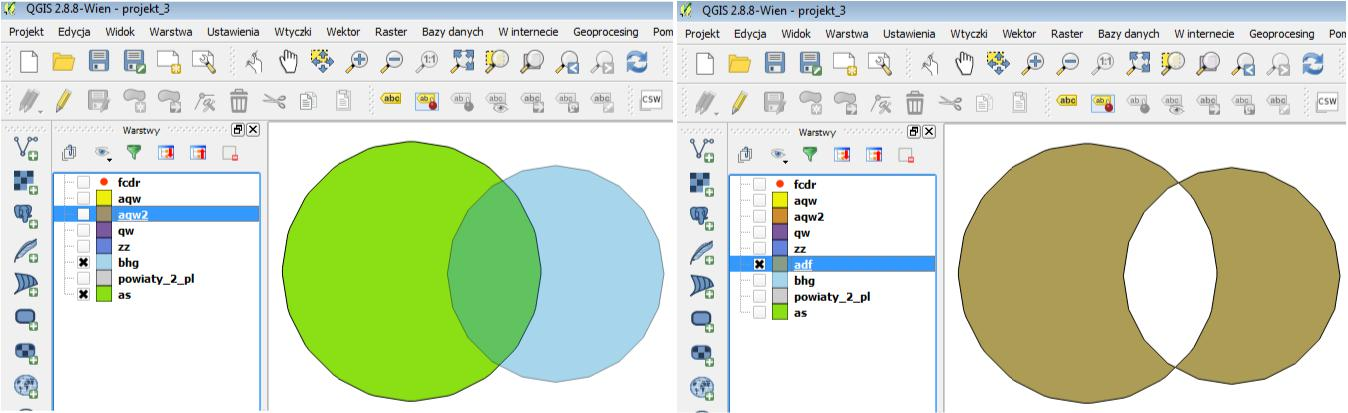
\includegraphics[width=16.365cm,height=5.009cm]{003-xor.jpg}
\caption{Wynik operacji Różnica Symetryczna}
\end{figure}
\end{center}
\item przytnij (clip) - przycina jedną warstwę do zasięgu innej warstwy; do tabeli zostają dołączone tylko atrybuty warstwy wejściowej (nie dołączają się atrybuty maski);
\item różnica (difference) - tworzy nowe obiekty, które są elementami obiektów warstwy wejściowej, które nie nakładają się na obiekty warstwy wycinającej; do tabeli zostają dołączone tylko atrybuty warstwy wejściowej;
\begin{center}
\begin{figure}
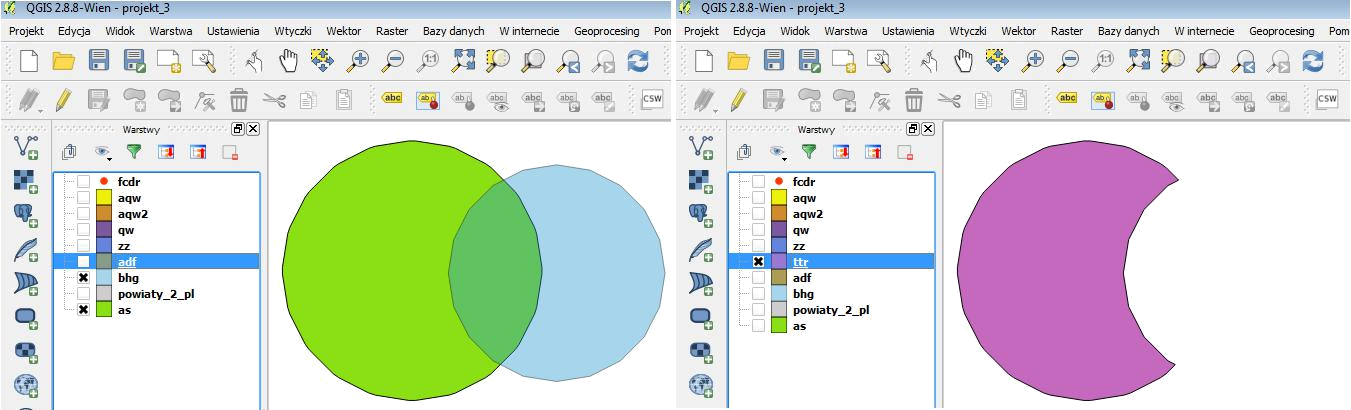
\includegraphics[width=16.365cm,height=4.967cm]{003-roznica.png}
\caption{Wynik operacji Różnica}
\end{figure}
\end{center}
\item agreguj (dissolve) - łączy pokrywające się obiekty danej warstwy w jeden obiekt;
\begin{center}
\begin{figure}
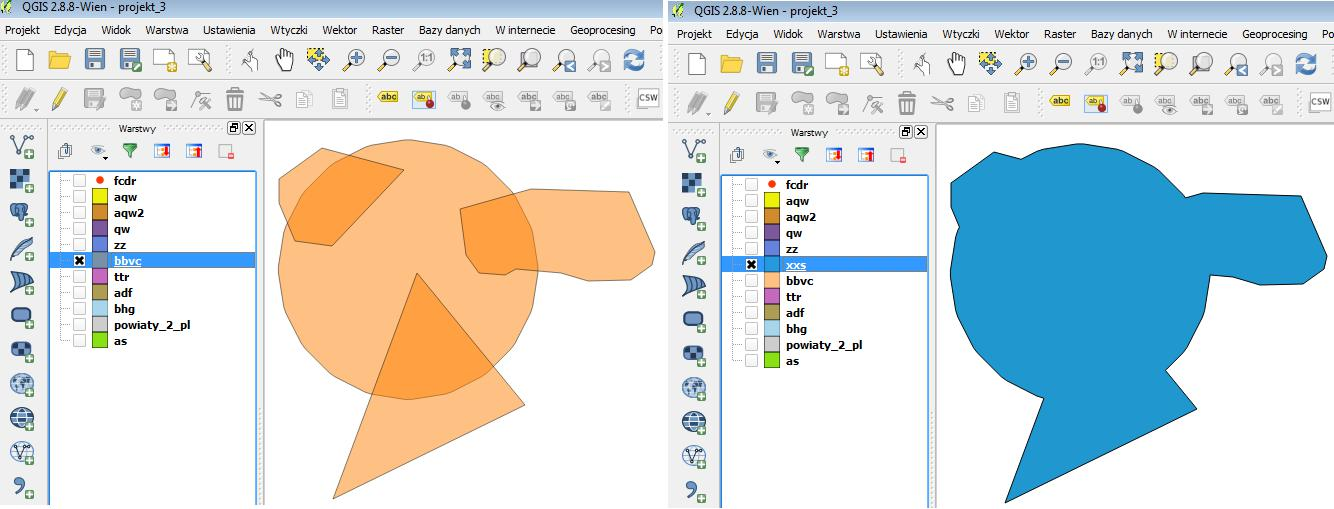
\includegraphics[width=16.365cm,height=6.244cm]{003-agreguj.jpg}
\caption{Wynik operacji Agreguj}
\end{figure}
\end{center}
\item eliminuj szczątkowe poligony - doąłcza małe obiekty do dużych w ramach jednej warstwy, jeśli się pokrywają.
\end{itemize}
\subsection{Operacje analityczne na warstwie}
Najprostszym narzędziem analitycznym dla warstw wektorowych w QGIS jest \textbf{Panel statystyk}. Dostęp do niego uzyskujemy poprzez menu  Widok-{\textgreater}Panele . Po uruchomieniu panelu, okno statystyk jest puste. Należy wybrać warstwę wektorową oraz pole atrybutowe dla którego mają być zliczane statystyki. Pole to pozwala na wprowadzenie wyrażeń dzięki którym możemy mieć dostęp np. do cech geometrii (powierzchnia, obwód, ilość segmentów linii, etc.)

\begin{center}
\begin{figure}
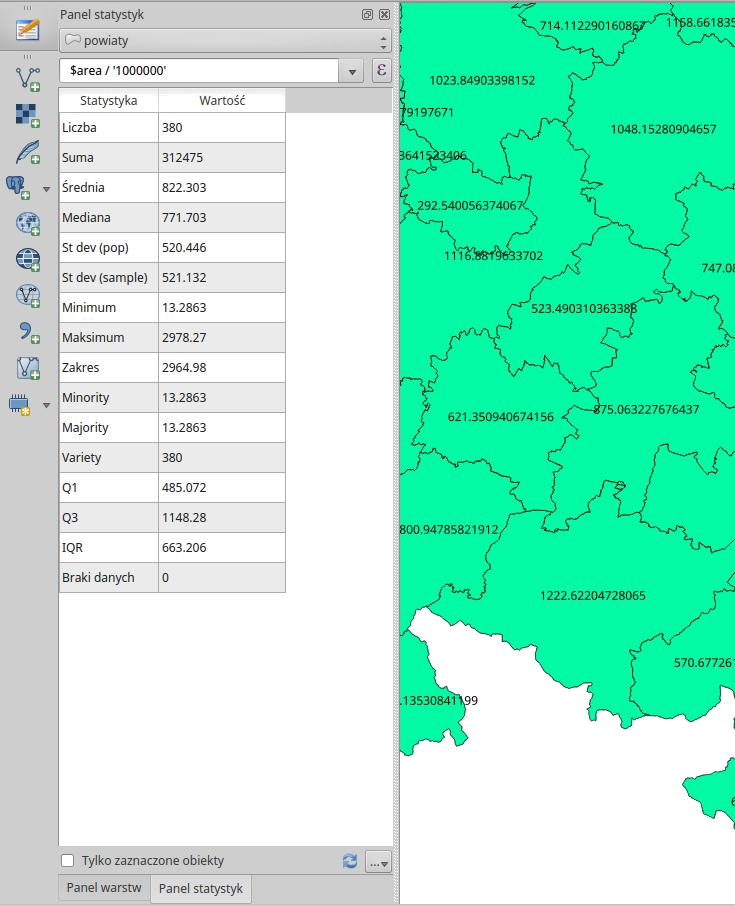
\includegraphics[width=13cm,height=16.013cm]{003-panel-stat.png}
\caption{Panel statystyk warstwy}
\end{figure}
\end{center}
Kolejne narzędzie to \textbf{Zlicz punkty poligonie} tworzy nową tabelę, z dodatkową kolumną (nazwę atrybutu należy określić samodzielnie), która zlicza ilość obiektów z warstwy punktowej zawierających się przestrzennie w obiektach warstwy poligonowej.

Następne przydatne narzędzie to \textbf{Group Stats. }Jest to rozszerzenie funkcjonalności QGIS o agregację i sumowanie klas. Możliwości takiego narzędzia zaprezentujemy na przykładzie warstwy gmin z Państwowego Rejestru Granic. Spróbujmy zaprezentować łączną powierzchnię gmin, wg typów jednostek (miejska, wiejska, mieszana).

Tak przygotowaną tabelę możemy wyeksportować do formatu CSV lub bezpośrednio skopiować do arkusza kalkulacyjnego.

\begin{center}
\begin{figure}
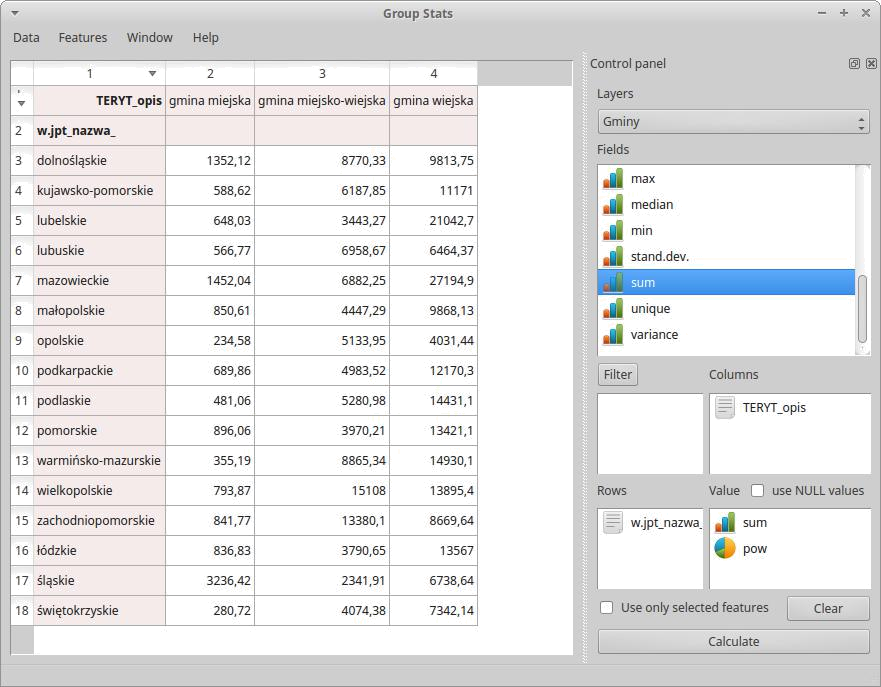
\includegraphics[width=17cm,height=13.222cm]{003-tabela-przestawna.png}
\caption{Tworzenie tabeli przestawnej - GroupStats}
\end{figure}
\end{center}
\subsection{Import CSV}
W przypadku konieczności przetworzenia danych do postaci przestrzennej, przydatne są funkcjonalności QGIS związane z otwieraniem arkusza kalkulacyjnego oraz pliku CSV bezpośrednio z poziomu aplikacji. Jeśli planujemy korzystać z danych tabelarycznych, bez geometrii, wystarczy użyć otwierania warstwy rastrowej i wybrać plik z dysku.

Inaczej sprawa wygląda gdy zamierzamy dokonać konwersji danych atrybutowych (współrzędnych) z tabeli na geometrię. W tym celu korzystamy z funkcji  Dodaj warstwę tekstową CSV  z panelu zarządzania warstwami.



\begin{center}
\begin{figure}
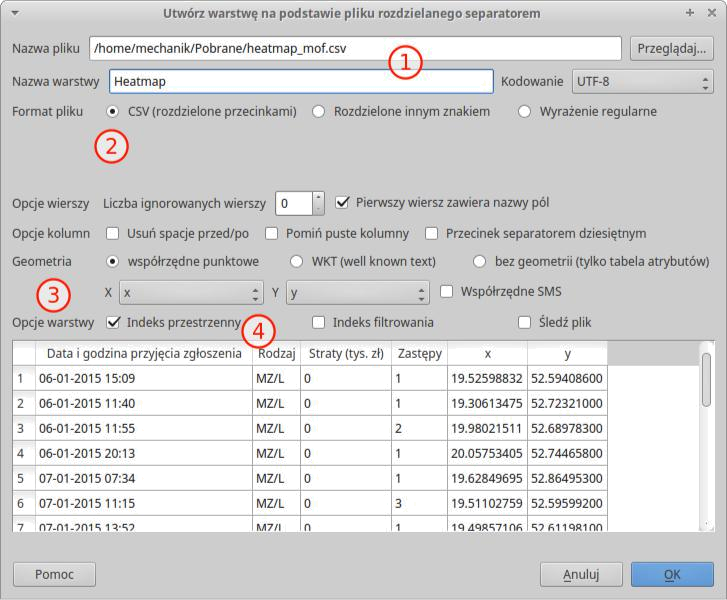
\includegraphics[width=13cm,height=10.696cm]{003-csv.png}
\caption{Opcje dodawania warstwy ze zbioru CSV}
\end{figure}
\end{center}
W otwartym oknie dialogowym, w pierwszej kolejności wybieramy plik z dysku, następnie wybieramy format pliku - możemy wskazać znak separatora pola. W pozycjach X i Y wskazujemy kolumny z tabeli w których znajdują się współrzędne. Czwórką oznaczony jest \textit{Indeks przestrzenny}.Tą opcję zawsze warto zaznaczyć, ponieważ przyśpiesza to potem dalszą pracę z taką warstwą (wyszukiwanie, zapytania i operacje przestrzenne).

Musimy pamiętać, że tak utworzona warstwa nie posiada zdefiniowanego układu współrzędnych i przypisywany jest układ domyślny dla nowych warstw. Koniecznym jest więc dostosowanie CRS do naszego zbioru danych.

\subsection{Relacje i złączenia}
Czasami natrafiamy na sytuację w której w zbiorze danych posiadamy pole atrybutowe o charakterze kodowym. Takim przykładem jest między innymi zbiór Corine Land Cover, czy zbiór TERYT:TERC. Aby umożliwić dostęp do informacji opisowej ze słownika powinniśmy skorzystać z operacji złączenia zbiorów danych. Systemy GIS pozwalają obecnie na dynamiczne złączenie (dopasowanie) na podstawie wybranej kolumny atrybutowej.

Tworząc nowe złączenie, w pierwszej kolejności otwieramy wszystkie konieczne zbiory danych, następnie z panelu warstw wybieramy **Właściwości warstwy**, tego zbioru który będzie warstwą rozbudowaną o pojęcia słownikowe. Na naszym przykładzie będzie to warstwa gmin z Państwowego Rejestru Granic. Złączymy kod TERYT województwa aby uzyskać jego nazwę, oraz typ jednostki administracyjnej, aby uzyskać parametr opisowy.. 

\begin{center}
\begin{figure}
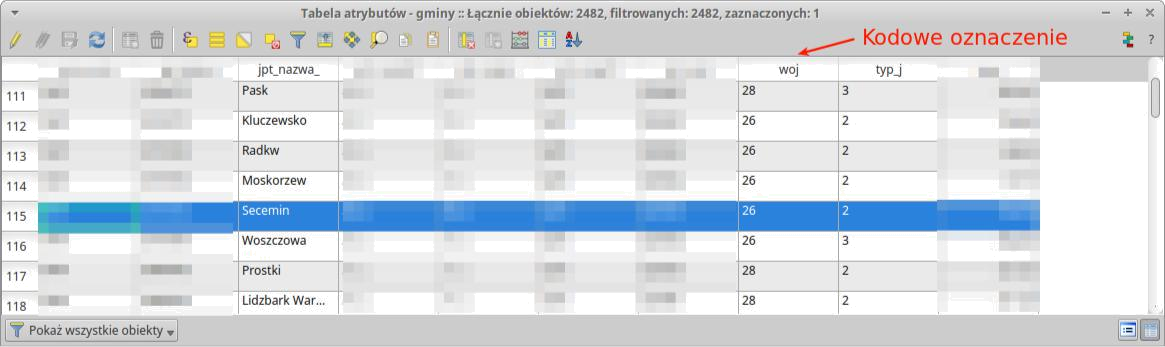
\includegraphics[width=17cm,height=5.059cm]{003-zlaczenia-atrybut.png}
\caption{Tabela atrybutów - atrybut do złączenia}
\end{figure}
\end{center}
Po otwarciu okna wybieramy zakładkę  Złączenia .

W lewym dolnym rogu znajduje się przycisk służący do tworzenia nowego złączenia. W otwartym oknie uzupełniamy kolejne pola. Dla pozycji \textit{Tabela} - \textit{Pole tabeli} wybieramy tabelę z której (zewnętrznej) będziemy dołączać, W pozycji \textit{Pole złączenia} wskazujemy pole w naszej tabeli podstawowej, do którego będzie dołączać po zgodnej wartości atrybutu.

Istnieje możliwość zaindeksowania pola złączenia, oraz wybrania pól z tabeli dołączanej, które ujawnią się w tabeli wynikowej. Przydatną jest również edycja pola prefiksu. Warto wybrać jedno-dwuznakowowy identyfikator, aby zaznaczyć pochodzenie danych. Po zatwierdzeniu i powrocie do okna mapy, sprawdzamy poprawność złączeń np. przy pomocy \textbf{Tabeli atrybutów}.



\begin{center}
\begin{figure}
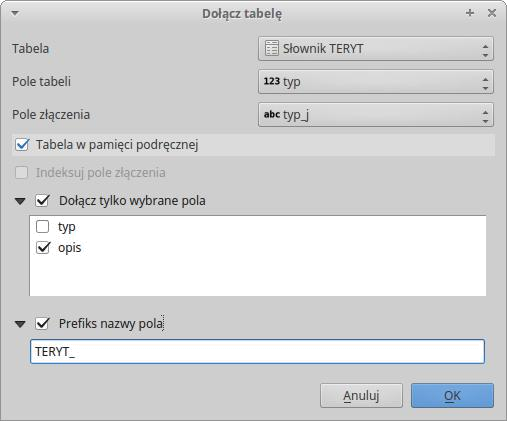
\includegraphics[width=11.998cm,height=9.952cm]{003-zlaczenie-edycja.png}
\caption{Edycja złączenia}
\end{figure}
\end{center}


\begin{center}
\begin{figure}
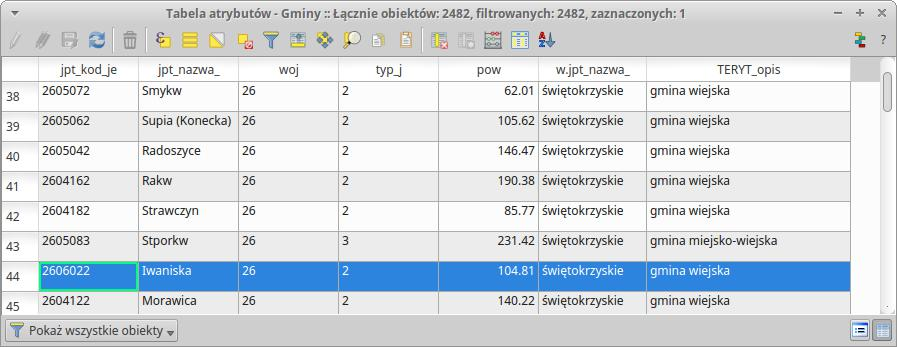
\includegraphics[width=17cm,height=6.548cm]{003-zlaczenie.jpg}
\caption{Złączona tabela}
\end{figure}
\end{center}
\subsection[Wyrażenia i kalkulator pól]{Wyrażenia i kalkulator pól}
Edycja dużej ilości danych może odbywać się za pomocą potężnego narzędzia analitycznego, jakim jest Kalkulator pól, które włączamy albo z poziomu tabeli albo z paska narzędzi.

Kalkulator pól umożliwia samodzielne wpisywanie wyrażeń lub posługiwanie się zdefiniowaną rozwijaną listą funkcji. Ponadto wybieramy i wskazujemy czy wykonane obliczenia (operacje) mają zostać zapisane w nowej kolumnie (jako nowy atrybut) czy tylko zaktulizować dane w już istniejącej kolumnie.

Jeśli chodzi o dostępne funkcje, to mamy do wyboru:

\begin{itemize}
\item \textbf{operatory}(dodawanie, odejmowanie, mnożenie, dzielenie, mniejsze/większe niż, itd.),
\begin{itemize}
\item LIKE – zwraca 1 jeśli pierwszy parametr odpowiada wzorcowi; wielkość liter ma znaczenie (alternatywą jest wyrażenie ILIKE, nie uwzględniające wielkości liter). Działa również na liczbach.
\item IS – zwraca 1 jeśli a i b są takie same.
\item OR – zwraca 1 przynajmniej jeden a lub b jest równe 1 (TRUE).
\item AND – zwraca 1, jeśli a i b są równe 1 (TRUE).
\item NOT – zwraca 1 jeśli a nie jest tożsame z b
\end{itemize}
\item \textbf{wyrażenia },\textbf{ warunkowe}
\item \textbf{pola i wartości} – zawiera listę atrybutów z danej warstwy, matematyczne - zawiera funkcje matematyczne (np. pierwiastek kwadratowy, sinus),
\item \textbf{konwersje}-ta grupaz awiera funkcje konwertujące dane pomiędzy różnymi typami (np. tekst na liczbę, liczbę na tekst),
\item \textbf{daty i czasu }zawiera funkcje do operowania na danych typu data i czas, tekstowe - zawiera funkcje do operowania na ciągach znaków (np. zamianie, konwersji czy zmianie wielkości liter),
\item \textbf{koloru }{}- zawiera funkcje do manipulowania kolorami,
\item \textbf{geometrii}{}-zawiera funkcje operujące na geometrii obiektów (np. długości, powierzchni,\textbf{ }buforach),
\item \textbf{wiersze }{}- ta grupa zawiera funkcje operujące na identyfikatorach wierszy,
\item \textbf{ostatnio użyte} – szybki skrót do ostatnio używanych funkcji.
\end{itemize}
Używany jest tu dialekt języka SQL, znacząco uproszczony i dostosowany do potrzeb programu.

Wyrażenia w QGIS mogą być wykorzystywane nie tylko w kalkulatorze pól i przy selekcji, ale również w czasie wizualizacji danych. Jest więc to bardzo praktyczna wiedza.

Przykładowe wyrażenie warunkowe

\texttt{CASE WHEN typ\_jednostki=WOJ THEN wojewoda ELSE premier END}

\subsection{Selekcja danych}
Przydatną kwestią jest umiejętność wybierania i zaznaczania obiektów na mapie. W menu Widok - Wybierz dostępnych jest kilka możliwych opcji:

\begin{itemize}
\item wybierz obiekty - zaznacza jeden lub wiele obiektów poprzez kliknięcie,
\item  wybierz obiekty wielobokiem - rysuje wielobok, który zaznacza obiekty, z którymi się przecina,
\item  wybierz obiekty zaznaczeniem - rysuje dowolny kształt, który zaznacza obiekty, które przecina,
\item wybierz obiekty promieniem - rysuje koło o dowolnym promieniu, które zaznacza obiekty, które przecina,
\item wybierz wyrażeniem - otwiera okno Select by expression (analogiczne do Kalkulatora pól), gdzie za pomocą wyrażenia zaznaczane są obiekty spełniające dany warunek,
\item zlikwiduj zaznaczenie obiektów ze wszystkich warstw - usuwa zaznaczenie wszystkich obiektów ze wszystkich warstw
\end{itemize}
\subsection{Tabela atrybutów}
Aby wyświetlić tabelę z atrybutami danej warstwy wektorowej należy w oknie panelu Warstwy kliknąć w nią prawym przyciskiem myszy i z menu podręcznego wybrać \textbf{Otwórz} \textbf{tabelę }.\textbf{atrybutów. }Z poziomu tego narzędzia można wykonać większość operacji zarządzania\textbf{ }strukturą tabeli danych, lecz dużo praktyczniejszym narzędziem pozostaje tutaj Table Manager.

\subsection{Edycja danych}
W celu dodania nowych obiektów, lub zmiany geometrii istniejących musimy przełączyć warstwę danych w tryb edycji. Następnie wybieramy narzędzie Dodaj obiekt, lub Edytuj.


\begin{center}
\begin{figure}
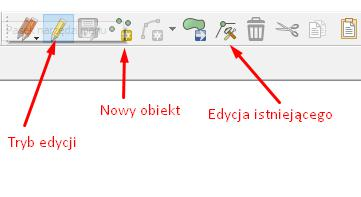
\includegraphics[width=8.901cm,height=4.851cm]{003-edycja.jpg}
\caption{Edycja danych}
\end{figure}
\end{center}
Każdorazowo aby móc skorzystać z wyedytowanych danych, konieczne jest ich zapisanie i wyłączenie trybu edycji, aby stały się w pełni dostępne dla pozostałych funkcji programu.


%Dane rastrowe
\chapter{Rastry}
\section{Łączenie rastrów}
\ \ Czasami zdarza się konieczność połączenia dwóch lub więcej zbiorów danych rastrowych. Może to być związane zarówno z potrzebą transformacji do innego układu współrzędnych, jak i połączenia wielu kanałów spektralnych obrazowań satelitarnych do postaci jednego zbioru.



\begin{center}
\begin{figure}
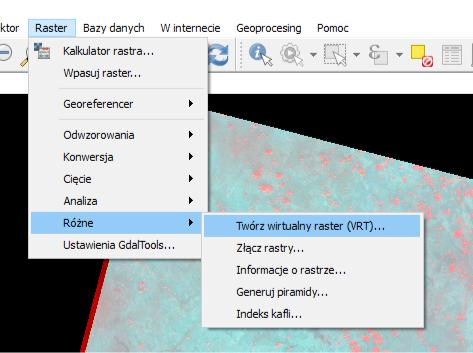
\includegraphics[width=12.513cm,height=9.338cm]{004-raster-rozne.jpg}
\caption{Menu Raster - Różne}
\end{figure}
\end{center}
\ \ Wszystkie te zadania możemy wykonać przy pomocy narzędzia znajdującego się w menu \textbf{Raster-{\textgreater}Różne-{\textgreater}Złącz rastry}

\ \ Jeśli zamierzamy wykorzystywać połączone kanały lub zasięgi głównie do wizualizacji, warto zrealizować te zadanie przy pomocy funkcji  Twórz wirtualny raster (VRT) . W ten sposób ilość zajętego miejsca na dysku nie rośnie znacząco.



\begin{center}
\begin{figure}
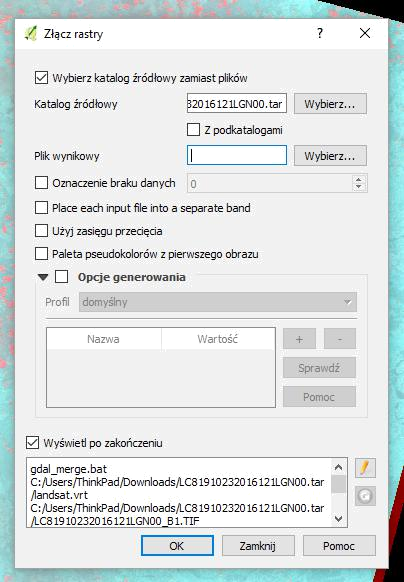
\includegraphics[width=10.689cm,height=15.402cm]{004-zlacz-rastry.png}
\caption{Operacja Złącz Rastry}
\end{figure}
\end{center}
Jeśli zamierzamy łączyć wiele rastrów znajdujących się w jednym katalogu, zaznaczamy pierwsze pole, następnie wskazujemy pliki/katalog źródłowy, ścieżkę do pliku wynikowego w którym zamierzamy zapisać. Kolejna ważna pozycja to  Place each input file into a seperate band  (Umieść każdy z plików w osobnym kanale). Używamy jej wyłącznie przy łączeniu wielu kanałów zobrazowań w jeden zbiór. W przypadku łączenia NMT, to pole powinno pozostać niezaznaczone.

\section{Kadrowanie rastrów}
\ \ Operacje na rastrach są dość obciążające obliczeniowo. Jeśli tylko jesteśmy w stanie, powinniśmy ograniczać wielkość zbioru rastrowego do niezbędnego minimum. Jednym ze sposobów jest ograniczanie zasięgu przestrzennego, przy pomocy narzędzi kadrowania rastrów. Narzędzia te znajdziemy w menu  Raster-{\textgreater}Cięcie .

\begin{center}
\begin{figure}
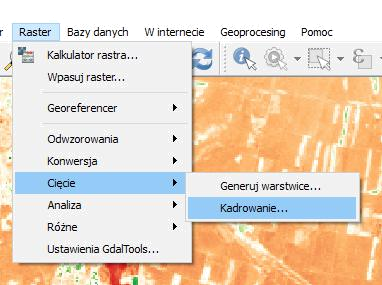
\includegraphics[width=10.111cm,height=7.542cm]{004-raster-ciecie.png}
\caption{Menu Raster - Cięcie}
\end{figure}
\end{center}

\begin{center}
\begin{figure}
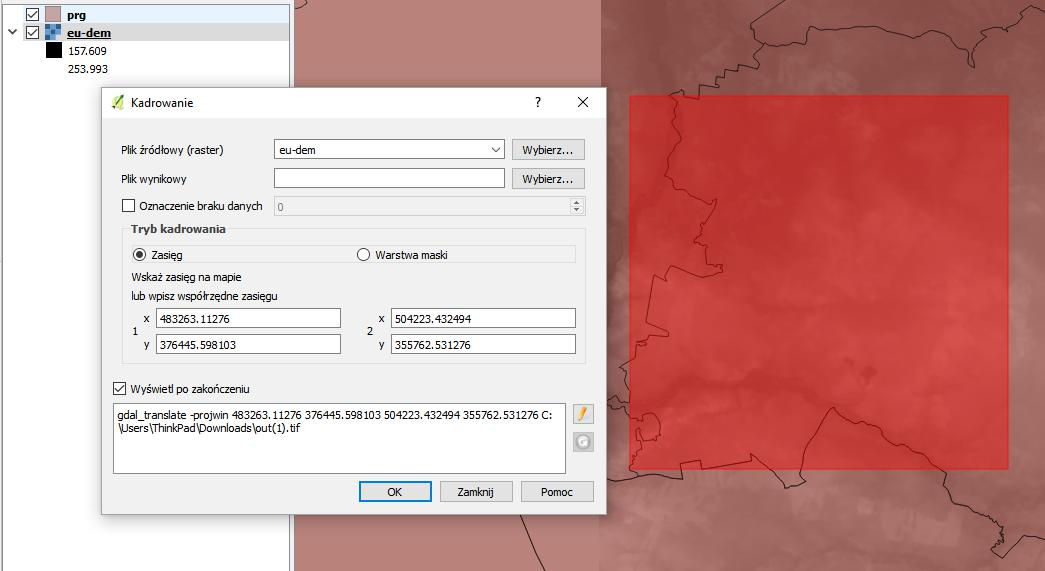
\includegraphics[width=13cm,height=7.091cm]{004-raster-kadrowanie.jpg}
\caption{Kadrowanie zasięgiem}
\end{figure}
\end{center}
\ \ W przypadku wyboru trybu kadrowania \textbf{Zasięg} należy pamiętać o ustawieniu układu CRS projektu zgodnego z układem warstwy rastrowej. Dla kadrowania przy pomocy \textbf{Warstwa maski} warstwa wektorowa musi mieć ten sam układ co raster, dla projektu możemy pozostawić układ wybrany do wizualizacji.

\begin{center}
\begin{figure}
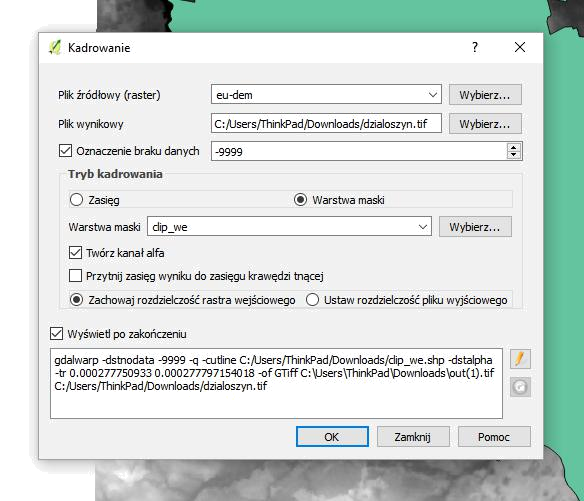
\includegraphics[width=15.452cm,height=13.229cm]{004-raster-maska.png}
\caption{Kadrowanie maską}
\end{figure}
\end{center}
Przydatnym jest również możliwość zdefiniowania wartości NODATA, oraz tworzenie kanału alfa (przezroczystości). Przykład takiego pliku na ilustracji.

\begin{center}
\begin{figure}
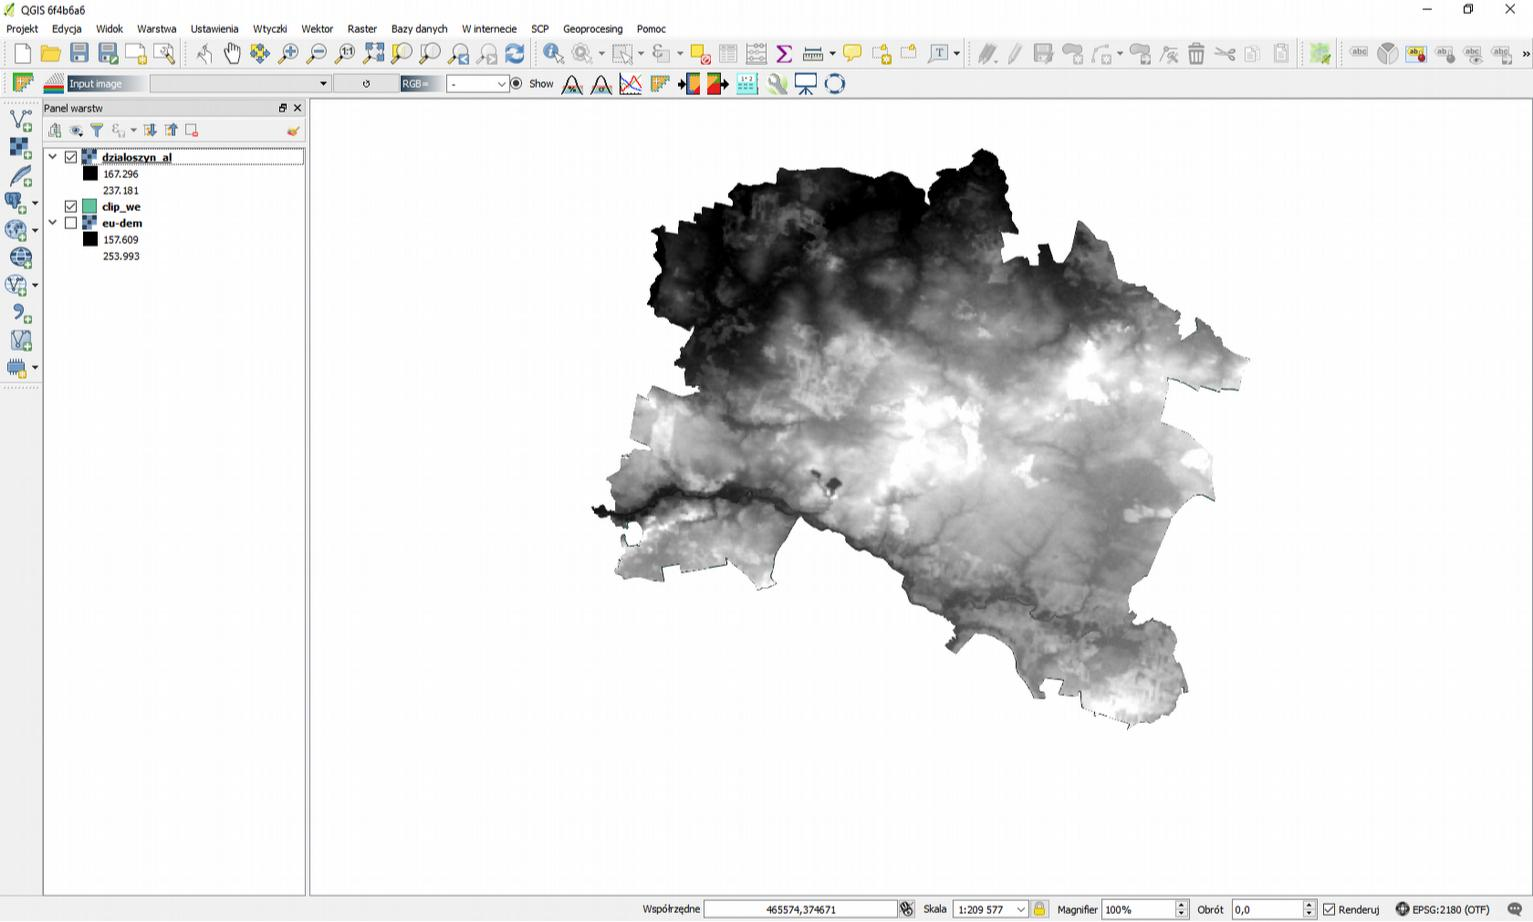
\includegraphics[width=13cm,height=7.796cm]{004-raster-alfa.jpg}
\caption{Kadrowanie maską z kanałem alfa} \label{fig:maskaalfa}
\end{figure}
\end{center}

\section{Opracowania multispektralne}
\ \ Przykładem wykorzystania obrazowań multispektralnych jest między innymi współczynnik NDVI. W QGIS można by go obliczać przy pomocy kalkulatora rastrów, lecz dużo praktyczniej skorzystać z gotowych narzędzi z pakietu SAGA.

\ \ Aby obliczyć NDVI, otwieramy warstwy rastrowe w osobnych kanałach, dla kanału 4 (bliska podczerwień) oraz kanału 3 (czerwony). Następnie przechodzimy do panelu  Geoprocessing  i wybieramy zakładkę  SAGA -{\textgreater}Image analysis , a następnie *Vegetation Index (slope based)*



\begin{center}
\begin{figure}
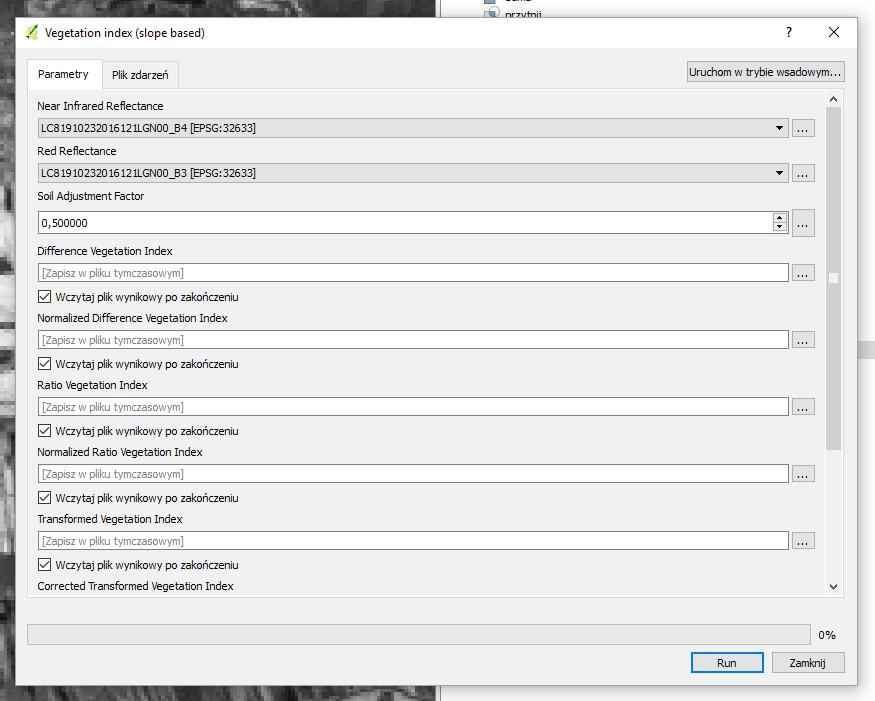
\includegraphics[width=13cm,height=10.389cm]{004-saga-ndvi.jpg}
\caption{Obliczanie indeksu NDVI}
\end{figure}
\end{center}
Uzupełniamy odpowiednie pola, wskazując kanały obrazu i zatwierdzamy klawiszem  Run .



\begin{center}
\begin{figure}
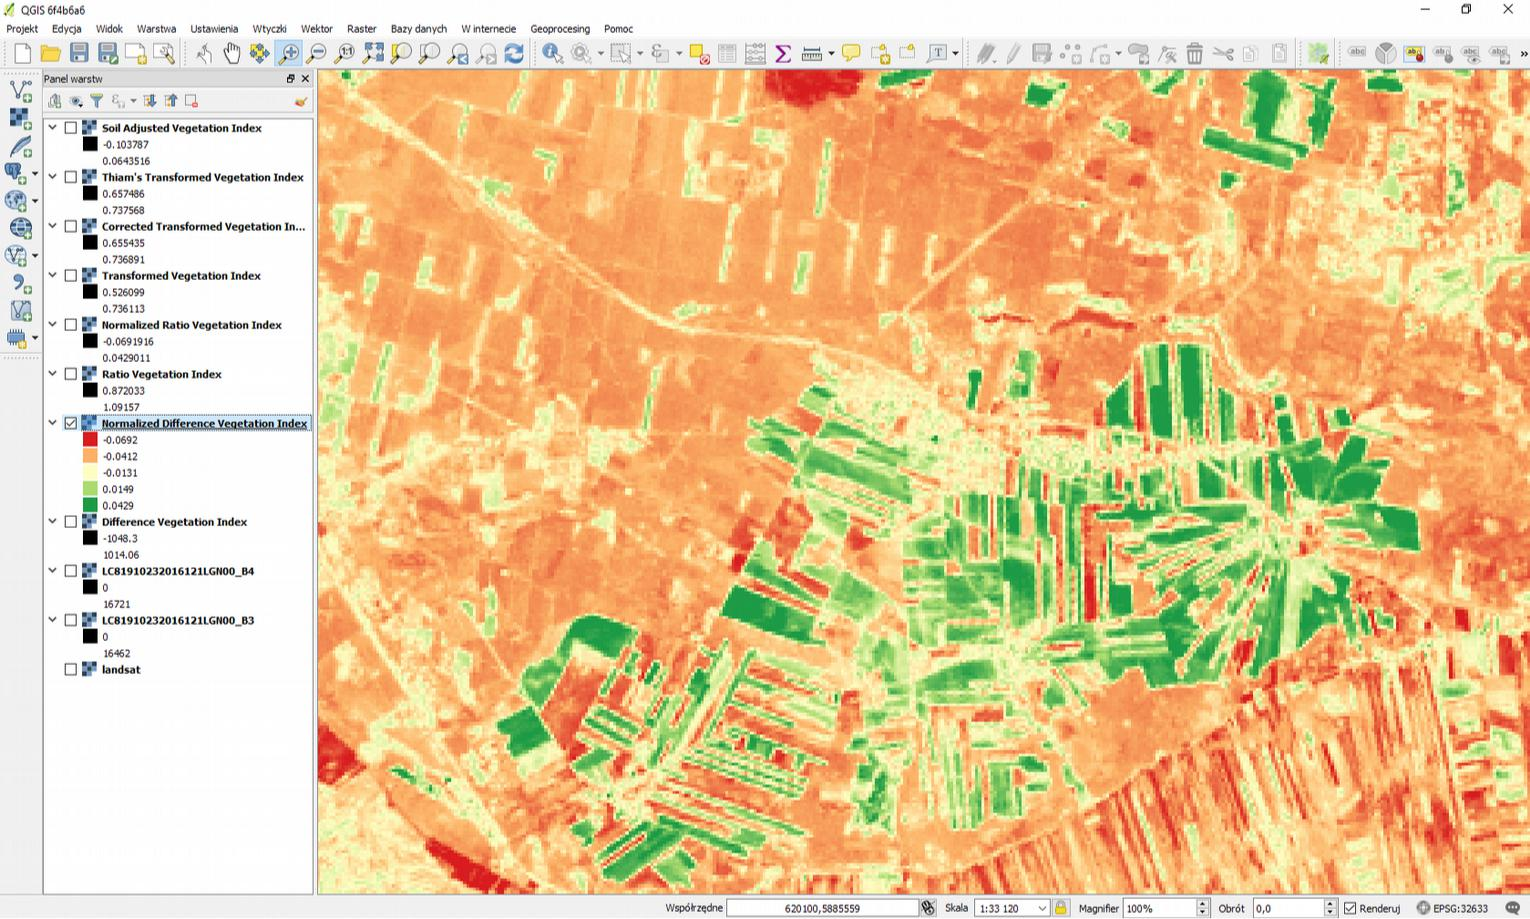
\includegraphics[width=13cm,height=7.786cm]{004-saga-grafika.jpg}
\caption{Wynik operacji obliczania NDVI}
\end{figure}
\end{center}
Wynikowy raster możemy zwizualizować lub zapisać do dalszego wykorzystania.

\section[Kalkulator rastra]{Kalkulator rastra}
Kalkulator rastra to narzędzie które pozwala na samodzielne opracowanie analityczne i obliczenia wartości punktów rastra, np. w sytuacji gdy dany algorytm czy metoda obliczeniowa nie została jeszcze zaimplementowana w oprogramowaniu GIS. W naszym przykładzie omówimy działanie kalkulatora przy pomocy wspomnianego w poprzednim rozdziale współczynnika NDVI.

Zastosujemy następujący wzór:
\begin{equation}
NDVI = \frac{NIR-VIS}{NIR+VIS}
\end{equation}
gdzie VIS to odbicie w paśmie czerwieni, zaś NIR odbicie w paśmie bliskiej podczerwieni.

Po wczytaniu interesujących nas warstw (w tym przykładzie zmieniono ich nazwy, dla zwiększenia czytelności), wybieramy menu  Raster-{\textgreater}Kalkulator rastra 


\begin{center}
\begin{figure}
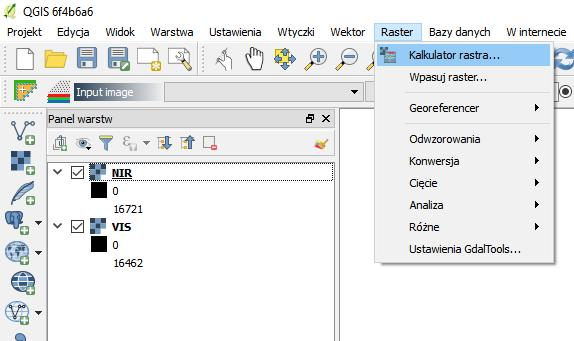
\includegraphics[width=13cm,height=7.691cm]{004-kalkulator.jpg}
\caption{Menu Raster - Kalkulator rastra}
\end{figure}
\end{center}
W oknie kalkulatora mamy możliwość wyboru z listy otwartych warstw rastrowych (lub ich kanałów), oraz operacji matematycznych. W dolnym oknie dialogowym wprowadzamy wyrażenie matematyczne.

\ \ Kalkulator rastra w module Geoprocessingu pozwala na wykorzystanie obliczeń bez tworzenia plików tymczasowych.

\begin{center}
\begin{figure}
\includegraphics[width=13cm,height=11.532cm]{004-kalkulator-ndvi.png}
\caption{Obliczanie NDVI w kalkulatorze rastra}
\end{figure}
\end{center}

\section{Numeryczny Model Terenu}
\subsection{Interpolacja rastra}
Jeśli dane wysokościowe jakimi dysponujemy istnieją tylko w postaci wektorowej, w pierwszej kolejności powinniśmy wykonać interpolację do postaci rastrowej. Dzięki dostępowi do narzędzi SAGA oraz GRASS, mamy możliwość skorzystania z kilku uznanych w środowisku naukowym metod interpolacyjnych, m.in.:

\begin{itemize}
\item Kriging
\item Thin plate Spline w odmianach zwykłej i TIN
\item Multilevel B-Spline
\item Metoda odwrotnych odległości
\item Metoda najbliższego sąsiedztwa
\end{itemize}
Technicznie operacja interpolacji w przypadku większości z tych metod jest bardzo podobna. Powinniśmy wskazać warstwę wektorową opisaną w oknie jako \textit{Points}, pole atrybutu, oraz rozmiar oczka siatki rastra \textit{Gridsize}.


\begin{center}
\begin{figure}
\includegraphics[width=9.446cm,height=9.525cm]{004-interpolacje.jpg}
\caption{Przykładowe narzędzia interpolacji}
\end{figure}
\end{center}
\begin{center}
\begin{figure}
\includegraphics[width=13cm,height=8.057cm]{004-kriging.jpg}
\caption{Algorytmy interpolacyjne - Kriging}
\end{figure}
\end{center}
\subsection{Preprocessing hydrologiczny}
Każdorazowo numeryczny model terenu utworzony przy pomocy interpolacji danych wektorowych, lub pochodzący ze zbiorów takich jak *SRTM, AsterDEM, EU-DEM* powinniśmy poddać procesowi usuwania zagłębień bezodpływowych (sink removal). Tu również z pomocą przychodzi nam pakiet SAGA, który w zakładce Terrain Analysis - Hydrology udostępnia kilka różnych wersji narzędzia, stosujących różne algorytmy. Wybór konkretnegoalgorytmu pozostawiam własnym doświadczeniom, lub rekomendacjom w literaturze. W naszym przykładzie skorzystamy z narzędzia opisanego jako \textbf{Sink removal}.


\begin{center}
\begin{figure}
\includegraphics[width=13cm,height=7.807cm]{004-pre-hydro.jpg}
\caption{Narzędzia preprocessingu hydrologicznego}
\end{figure}
\end{center}
Pozwala nam on dostosować metodę usuwania zagłębień na dwa sposoby - poprzez pogłębianie kanałów spływu powierzchniowego, lub poprzez {\textquotedbl}zasypywanie{\textquotedbl}.



\begin{center}
\begin{figure}
\includegraphics[width=13cm,height=10.456cm]{004-sink.jpg}
\caption{Sink removal - ustawienia}
\end{figure}
\end{center}
\subsection{Kanały spływu powierzchniowego, zlewnie}
Kolejne operacje które możemy wykonać przy pomocy narzędzi geoprocessingu to wyznaczenie kanałów spływu powierzchniowego, oraz zlewni. Znajdziemy je w zakładce \textbf{Terrain Analysis - Channels}.



\begin{center}
\begin{figure}
\includegraphics[width=9.338cm,height=8.255cm]{004-saga-anali.jpg}
\caption{Narzędzia analityczne SAGA}
\end{figure}
\end{center}
W wyniku tej operacji możemy otrzymać warstwy wektorowe dla zlewni i kanałów, czy rastrowe warstwy określające kierunek spływu powierzchniowego.

\begin{center}
\begin{figure}
\includegraphics[width=13cm,height=10.587cm]{004-saga-splyw.jpg}
\caption{Kanały spływu powierzchniowego - obliczenia}
\end{figure}
\end{center}
\subsection{Morfometria rzeźby terenu}
W zakładce \textbf{Terrain analysis morphometry }znajdziemy zgrupowane ważniejsze narzędzia i algorytmy do obliczeń cech morfometrycznych rzeźby terenu takich jak nachylenie stoku, ekspozycja, krzywizny, wskaźnik TRI.



\begin{center}
\begin{figure}
\includegraphics[width=8.597cm,height=11.709cm]{004-morfo.jpg}
\caption{Analizy morfometryczne}
\end{figure}
\end{center}
\subsection{Tworzenie warstwic}
%Problem
Jeśli potrzebujemy stworzyć dla celów wizualizacji warstwę wektorową, z przebiegiem warstwic, korzystamy w tym celu z narzędzia znajdującego się w menu Raster - Cięcie i wybieramy pozycję Generuj warstwice. Następnie wskazujemy przy pomocy myszy Wybierz plik docelowy,. jak również zaznaczymy pole \textbf{Nazwa atrybutu }i wprowadzamy naszą nazwę pola. W polu \textbf{Cięcie warstwicowe }ustawiamy parametr cięcia, odstępu wysokościowego pomiędzy kolejnymi\textbf{ }warstwicami.


\begin{center}
\begin{figure}
\includegraphics[width=15.004cm,height=9.578cm]{004-warstwice-opcje.jpg}
\caption{Opcje tworzenia cięcia warstwicowego}
\end{figure}
\end{center}


\begin{center}
\begin{figure}
\includegraphics[width=14.997cm,height=8.971cm]{004-warstwice-wynik.jpg}
\caption{Wynik operacji - Cięcie warstwicowe}
\end{figure}
\end{center}
\section{Georeferencja map archiwalnych}
\ \ QGIS udostępnia możliwość wprowadzenia danych o powiązaniu przestrzennym zeskanowanego archiwalnego arkusza mapy. W tym celu korzystamy z narzędzia \textbf{Georeferencer GDAL }znajdującego się w menu\textbf{ }Raster.



\begin{center}
\begin{figure}
\includegraphics[width=9.899cm,height=8.149cm]{004-georef.jpg}
\caption{Narzędzie georeferencji}
\end{figure}
\end{center}


\begin{center}
\begin{figure}
\includegraphics[width=14.997cm,height=11.539cm]{004-georef-okno.jpg}
\caption{Georeferencer - okno robocze}
\end{figure}
\end{center}
Po otwarciu okna wtyczki ujrzymy górny pasek narzędzi. Na powyższej ilustracji cyfrą jeden oznaczono \textbf{Otwieranie pliku rastrowego, }bez georeferencji.Następnie powinniśmy skorzystać z przycisku \textbf{Ustawienia }oznaczonego cyfrą trzy. W oknie ustawień zdefiniujemy parametry transformacji (zarówno transformacji geometrycznej arkusza, jak i transfomracji układu wspórzędnych), a także wskażemy docelowy plik rastrowy.



\begin{center}
\begin{figure}
\includegraphics[width=13cm,height=13.702cm]{004-georef-transf.jpg}
\caption{Ustawienia parametrów transformacji rastra}
\end{figure}
\end{center}
Cyfrą cztery oznaczone są narzędzia dodawania, edycji i usuwania punktów kontrolnych. Warto zaznaczyć że pozwalają one zarówno na wprowadzanie współrzędnych zgodnych z układem oryginalnym, jak i korzystanie z innej mapy/zdjęcia lotniczego w oknie głównym QGIS i wskazywanie takich punktów bezpośrednio na mapie.

W dolnej części okna znajdziemy listę punktów kontrolnych wraz z informacją o błędzie lokalizacji dla każdego z nich, umożliwia to ocenę dokładności spozycjonowania mapy, przed wykonaniem transformacji do postaci docelowej, przy pomocy przycisku oznaczonego cyfrą dwa.


%Rozdział Przetwarzanie LiDARu
\chapter{LiDAR}
Rozwój technologii pozwala nam na coraz to większe możliwości teledetekcyjne. Jednym z takich rozwiązań jest LiDAR. Rozwiązania lotniczego i naziemnego skaningu laserowego pozwalają na szybkie i mniej pracochłonne tworzenie numerycznego modelu terenu, czy opracowań związanych z pokryciem, zagospodarowaniem przestrzennym, a także coraz aktywniej rozwijane aplikacje detekcji zmian rzeźby.

W naszych przykładach będziemy operować na algorytmach wbudowanych w pakiet LASTools, pamiętając o tym że nie wszystkie jego funkcjonalności są udostępnione na licencji open-source/freeware. Niektóre wymagają licencji komercyjnej/naukowej.

\section{Klasyfikacja}
Jeśli dane LiDAR nie zostały wcześniej sklasyfikowane, konieczne jest użycie kiku kolejno po sobie następujących narzędzi. Najwygodniej uczynić to przy pomocy Modelarza z rozszerzenia  Geoprocessing . Przykładowy ciąg operacji znajduje się na ilustracji poniżej.



\begin{center}
\begin{figure}
\includegraphics[width=13cm,height=7.691cm]{005-model-chmura.jpg}
\caption{Przetwarzanie modelowe - Klasyfikacja chmury punktów}
\end{figure}
\end{center}
W kolejnych krokach wprowadzamy do podstawowego zbioru dodatkowe informacje, które pozwolą na pełne wykorzystanie chmury i wykonanie szerszego zbioru analiz. W pierwszej kolejności, przy pomocy  lasground  znajdujemy punkty które odpowiadają powierzchni gruntu. Istotną zmienną jest tu charakter terenu (nature, wilderness, city, town, metro) - są to predefiniowane współczynniki zmienności terenu w danych warunkach otoczenia. Następnie  lasheight  oblicza i wprowadza do zbioru w polu  user data  dodatkową informację o wysokości danego punktu ponad powierzchnią gruntu. Tu możemy zdecydować o odrzuceniu ze zbioru punktów które są położone powyżej (-drop-above) lub poniżej (-drop-below) zdefiniowanego progu w stosunku do powierzchni. Na tej podstawie  lasclassify  analizuje sąsiedztwo punktów i przydziela je do odpowiednich klas. Tak przygotowany plik LAS może nam posłużyć do dalszych prac.

\section{Pokrycie terenu}
Przy pomocy  lasboundary  z pakietu LASTools można pozyskać zasięgi przestrzenne pokrycia terenu daną klasą chmury punktów. Korzystając z docku Geoprocessing wybieramy \textbf{Narzędzia do danych LiDAR }z listy narzędzi lasboundary \textbf{LASTools.}



\begin{center}
\begin{figure}
\includegraphics[width=13cm,height=9.126cm]{005-lasboundary.jpg}
\caption{LasBoundary - Wyznaczanie zasięgów klasy}
\end{figure}
\end{center}
W widocznym oknie uzupełniamy kolejno parametry algorytmu. W polu oznaczonym cyfrą jeden wprowadzamy źródłową chmurę punktów z klasyfikacją.

Jeśli chcemy skorzystać z zdefiniowanego filtra, wybieramy jego wartość w liście oznaczonej cyfrą dwa. W polu  concavity  oznaczonym cyfrą trzy możemy zmienić promień poszukiwań dla otoczki wklęsłej. Jego zmniejszanie powoduje zwiększenie ilości tworzonych obiektów. Pole oznaczone cyfrą cztery pozwala na stworzenie wielu osobnych poligonów, lub jednego połączonego. W polu  additional command line parameters  możemy wprowadzić dodatkowe wymagania. W naszym przykładzie zrezygnujemy z definicji filtra, na rzecz samodzielnego  -keep\_class 5 , a więc wybrania wyłącznie klasy wysokiej wegetacji.

\begin{center}
\begin{figure}
\includegraphics[width=13cm,height=9.426cm]{005-klasy.png}
\caption{Efekt selekcji dla klas 3,4,5, osobno dla klasy 5 oraz dla klasy 6}
\end{figure}
\end{center}

\section{Numeryczny model terenu}
Narzędziem służącym konwersji chmury punktów do formatu rastrowego jest  las2dem .

\begin{center}
\begin{figure}
\includegraphics[width=13cm,height=12.771cm]{005-lasdem.jpg}
\caption{Okno parametrów przetwarzania las2dem}
\end{figure}
\end{center}
W przypadku tego narzędzia najistotniejsze parametry to:

\begin{itemize}
\item step size/pixel size (rozmiar oczka rastra wynikowego)
\item atrybut
\item produkt
\end{itemize}


\begin{center}
\begin{figure}
\includegraphics[width=13cm,height=2.72cm]{005-atrybut.jpg}
\caption{Możliwości wartości wynikowe atrybutu}
\end{figure}
\end{center}


\begin{center}
\begin{figure}
\includegraphics[width=13cm,height=1.831cm]{005-produkt.jpg}
\caption{Możliwość wyboru produktu las2dem}
\end{figure}
\end{center}

\begin{center}
\begin{figure}
\includegraphics[width=13cm,height=9.419cm]{005-lasdem-wynik.jpg}
\caption{Wynikowe opracowanie las2dem}
\end{figure}
\end{center}

% Rozdział Zarządzanie bazą danych
\chapter{Baza danych}
\section{PostgreSQL}
PostgreSQL to obecnie najbardziej rozbudowany silnik bazy danych w środowisku open-source. Jego dynamiczny rozwój, oraz wiele funkcjonalności „enterprise” powoduje coraz szersze wykorzystanie nie tylko w pracach akademickich, ale również w wielu światowych korporacjach. Powstał jako projekt relacyjnej bazy danych w 1986 roku na University of California w Berkeley (UCB). Twórcą jego założeń był Michael Stonebraker, a w 1995 przebudowy dokonali doktoranci Andrew Yu i Jolly Chen. W maju 2001 firma Refractions wydała na licencji zgodnej z PostgreSQL rozszerzenie przestrzenne PostGIS. Pod koniec tego samego roku rząd Kolumbii Brytyjskiej sfinansował prace nad biblioteką Java Topology Suite, która po niewielkich zmianach stała się podstawą funkcji relacji przestrzennych PostGIS’a, oraz biblioteki GEOS wykorzystywanej przez QGIS’a. Warto też zaznaczyć że pierwsza wersja QGIS obsługiwała wyłącznie bazy danych PostGIS jako źródło danych przestrzennych.

\section{SQLite/Spatialite}
Powstał w 2000 roku jako silnik plikowej bazy danych. W przeciwieństwie do Postgres’a, każda z baz danych SQLite jest osobnym plikiem, który potencjalnie można skopiować i rozpocząć jego używanie w innym środowisku. To oraz wydajność pracy silnika przy jednym użytkowniku stanowią o popularności SQLite w . W 2008 roku powstało rozszerzenie przestrzenne Spatialite. W 2013 roku OGC przyjęło nowy standard przechowywania danych przestrzennych GeoPackage, oparty o strukturę binarną pliku bazy bazy danych Spatialite.

\section{Podstawowe zapytania}
Składnia PostgreSQL jest oparta o budowę zdania w języku angielskim,

SELECT (kolumny) FROM schema.tabele WHERE warunek ORDER BY kolejnosc;

Każde zdanie (zapytanie) powinno się kończyć średnikiem. W jednym przebiegu można wykonać wiele zapytań. Przy tym * (gwiazdka) oznacza wybór wszystkich kolumn ze wszystkich wskazanych tabel. Warto pamiętać że w środowisku psql dla wykonania zapytania do pamięci zaczytane zostaną wszystkie wskazane kolumny, a więc jeśli to niekonieczne, warto literalnie wskazać wymagane przez nas kolumny atrybutów które mają znaleźć się w tabeli wynikowej, oraz korzystać z „funkcji okienkowej” WITH, która przygotowuje wstępną tabelę tymczasową z wymaganymi przez nas danymi.

Baza danych PostgreSQL pozwala na przechowywanie tabel w tzw. schematach (schema). Schema to odpowiednik katalogu w systemie plików.

\section{Operacje przestrzenne}
Operacje przestrzenne w środowisku Postgresql/PostGIS realizowane są przy pomocy funkcji o nazwach poprzedzonych przedrostkiem ST\_. Do najczęściej wykorzystywanych należą ST\_Union, ST\_Buffer, ST\_Intersects, ST\_Touches.

\subsection{ST\_Distance()}
Służy do pomiaru odległości pomiędzy dwoma obiektami. Zwraca minimalną odległość kartezjańską.

\begin{verbatim}
WITH
poznan AS (SELECT geometry FROM powiaty WHERE nazwa=’Poznań’) chorzow AS (SELECT geometry FROM powiaty WHERE nazwa=’Chorzów’)
SELECT ST_Distance(poznan.geometry, chorzow.geometry);
\end{verbatim}
\subsection{ST\_Intersects()}
Sprawdza czy obiekty mają część wspólną. Dla funkcji powinniśmy podać dwie geometrie, przy czym pierwsza z nich powinna być pojedyńczym obiektem (lub jego unią).

\begin{verbatim}
WITH
poznan AS (SELECT geometry FROM powiaty WHERE nazwa=’Poznań’) woda AS (SELECT geometry FROM hydranty)
SELECT ST_Intersects(poznan.geometry, woda.geometry);
\end{verbatim}
\subsection{ST\_Buffer()}
\ \ Tworzy otoczki o zadanym promieniu wokół obiektów. ST\_Buffer potrafi przyjąć jako argument dla promienia wartość zerową lub ujemną, co ma swoje praktyczne zastosowanie. W przypadku wartości ujemnej obiekt poligonowy zostanie zmniejszony, zaś w przypadku wartości zerowej, zostanie przebudowana geometria obiektu. Jest to przydatna funkcjonalność w przypadku problemów z topologią geometrii.

\begin{verbatim}
SELECT ST_Buffer(geometry, 75) FROM hydranty;
\end{verbatim}
\section{Operacje analityczne}
Operacje analityczne w środowisku psql realizowane są przy pomocy funkcji agregacyjnych, oraz sortujących, takich jak sum(), count(), oraz operacji ORDER BY, GROUP BY.

\subsection{SUM()}
Wykonuje sumowanie wartości dla wskazanej kolumny. Przykładowo możemy zsumować liczbę ludności powiatów, sortując ją wg województwa.

\begin{verbatim}
SELECT nazwa_wojewodztwa, SUM(ludnosc) FROM powiaty GROUP BY nazwa_wojewodztwa;
\end{verbatim}
\subsection{COUNT()}
Jest najprostszą funkcją agregującą, zlicza wystąpienie danego warunku. Przykładowo zliczmy ilość powiatów w województwach.

\begin{verbatim}
SELECT nazwa_wojewodztwa, COUNT(*) FROM powiaty GROUP BY nazwa_wojewodztwa;
\end{verbatim}
Pozostałe funkcje agregacyjne to AVG(), MIN(), MAX(), ARRAY().

\section{Warstwy wirtualne}
W QGIS od wersji 2.14 pojawiło się nowe narzędzie Warstwa wirtualna, które pozwala na udostępnienie funkcji bazodanowych Spatialite z poziomu interfejsu QGIS, bez konieczności tworzenia i importu do bazy. Jednocześnie dzięki temu możemy uniknąć tworzenia wielu warstw pośrednich dla przetworzenia danych.


\begin{center}
\begin{figure}
\includegraphics[width=13cm,height=9.917cm]{006-virtual.jpg}
\caption{Warstwa wirtualna}
\end{figure}
\end{center}
Po otwarciu okna przy pomocy klawisza \textbf{Importuj }dodajemy do warstwy wirtualnej istniejące warstwy danych z projektu. Istnieje również możliwość ich dodania bezpośrednio z dysku, lecz wymaga to ręcznego wpisania pełnej ścieżki dostępu do danych. Następnie w oknie \textbf{Zapytanie }wprowadzamy zapytanie w dialekcie Spatialite. Klawiszem\textbf{ Testuj }możemy sprawdzić poprawność zapytania, a następnie klawiszem \textbf{OK}wykonać operację i dodać wynik do okna głównego.

\chapter{Stylizacja warstw}
Choć systemy informacji geograficznej, a QGIS nie jest tu wyjątkiem, powstały głównie w celach analitycznych, w ostatnich latach posiadają coraz więcej narzędzi do wizualizacji kartograficznej. W przypadku naszego środowiska te zmiany są szczególnie aktywne w ostatnim okresie i choć wciąż dodawane są nowe moduły dla celów obliczeniowych, głównie w oparciu o Processing, to wysyp funkcjonalności dla kartografów, czyni QGIS'a liderem wśród pakietów open-source.

Aby rozpocząć wizualizację warstwy danych, w panelu warstw prawym klawiszem myszy uzyskujemy dostęp do menu kontekstowego, wybierając \textbf{Właściwości warstwy.}



\begin{center}
\begin{figure}
\includegraphics[width=11.596cm,height=12.771cm]{007-kontekstowe.jpg}
\caption{Menu kontekstowe - Właściwości warstwy}
\end{figure}
\end{center}
W otwartym oknie wybieramy zakładkę styl. Od wersji 2.16 możliwe jest również skorzystanie z panelu Styl mapy. Aby go aktywować należy wybrać menu  Widok -{\textgreater} Panele  i odpowiedni panel.

\section{Raster}
\ \ We właściwościach warstwy rastrowej możemy znaleźć zakładkę Styl w której znajdziemy następujące ustawienia:



\begin{center}
\begin{figure}
\includegraphics[width=13cm,height=2.868cm]{007-raster-tryby.jpg}
\caption{Tryby renderowania warstwy rastrowej}
\end{figure}
\end{center}
\subsection{Kolor wielokanałowy}
Ta opcja służy do przygotowania wizualizacji obrazów multispektralnych, takich jak zdjęcia satelitarne. W przypadku takich zdjęć wykonywanych w wielu kanałach spektralnych, każdy z kanałów prezentuje 32 bitową paletę odcieni szarości. Dopiero połączenie trzech kanałów powoduje wizualizację w przestrzeni barwnej RGB. ![Właściwości kolor wielokanałowy] (wlasciwosci\_kolor\_wielokanalowy.png)

\ \ Na ilustracji powyżej widzimy przykładowe ustawienia dla obrazów Landsat, z wykorzystaniem obrazowania podczerwieni. Koniecznym jest również wykorzystanie pozycji **Wzmocnienie kontrastu** z ustawieniem **Rozciągnij do min./max.** lub **Rozciągnij i przytnij**. Powodują one zwiększenie kontrastu obrazu.

\subsection{Paleta barw}
Ten tryb pozwala na wczytanie wcześniej przygotowanej palety barwnej.

\subsection{Jednokanałowy szary}
Wizualizacja trybem jednokanałowy-szary może być przydatna dla prezentacji cech o niewielkiej zmienności.



\begin{center}
\begin{figure}
\includegraphics[width=11.613cm,height=11.01cm]{007-raster-jedno.png}
\caption{Tryb renderowania jednokanałowego w skali szarości}
\end{figure}
\end{center}
\begin{center}
\begin{figure}
\includegraphics[width=13cm,height=9.723cm]{007-raster-szary.jpg}
\caption{Jednokanałowy szary - wygląd}
\end{figure}
\end{center}
\subsection{Jednokanałowy pseudokolor}
\ \ Ten typ wizualizacji jest szczególnie przydatny w przypadku numerycznego modelu terenu i jego produktów pochodnych. Możemy dzięki nim przedstawić mapę w postaci hipsometrycznej, czy zaprezentować zjawiska spadków, krzywizn szczególnie intuicyjnymi kolorami.



\begin{center}
\begin{figure}
\includegraphics[width=13cm,height=9.666cm]{007-raster-pseudo.jpg}
\caption{Wizualizacja jednokanałowa z paletą barwną}
\end{figure}
\end{center}
W tym przypadku mamy również większy wpływ na ostateczny kształt wizualizacji. Na kolejnych ilustracjach przedstawiona została wizualizacja tego samego zbioru danych, w oparciu o tą samą paletę barwną.

\begin{center}
\begin{figure}
\includegraphics[width=17cm,height=11.529cm]{007-raster-dyskretna.png}
\caption{Dyskretna paleta barwna}
\end{figure}
\end{center}
\begin{center}
\begin{figure}
\includegraphics[width=17cm,height=11.546cm]{007-raster-liniowa.jpg}
\caption{Liniowa paleta barwna}
\end{figure}
\end{center}
\subsection{Hillshade renderer}
Ta opcja dostępna jest wyłącznie od wersji 2.15/2.16 wzwyż. W wcześniejszych wersjach programu konieczne było przygotowanie pliku TIFF wywołując z menu Raster -{\textgreater} Analiza -{\textgreater} Numeryczny Model Terenu. Od wersji 2.16 takie cieniowanie rzeźby terenu może być tworzone dynamicznie, wraz z możliwością dostosowania parametrów wizualizacji w czasie rzeczywistym.

\section{Wektor}
\ \ Dla warstw wektorowych mamy możliwość skorzystania z wielu różnych rendererów, które umożliwą zaprezentowanie zarówno treści kartogramu, jak i typowej mapy topograficznej.



\begin{center}
\begin{figure}
\includegraphics[width=7.938cm,height=3.81cm]{007-wektor-tryby.jpg}
\caption{Tryby wizualizacji wektorowej}
\end{figure}
\end{center}

\subsection{Jeden symbol}
\ \ Podstawowy sposób wyświetlania nowo otworzonej warstwy. Wszystkie obiekty zostaną wyświetlone identycznym symbolem, który może mieć postać markera punktowego, wypełnień stałych lub gradientowych, obrysów. Każdy z tak utworzonych symboli może być ponownie wykorzystany, również w każdym pozostałym trybie wizualizacji. 

\subsection{Wartośc unikalna}
\ \ Przy pomocy tej funkcji możemy zaprezentować zdefiniowane (dyskretne) wartości atrybutów za pomocą symbolu o zmiennej kolorystyce.

\begin{center}
\begin{figure}
\includegraphics[width=13cm,height=12.746cm]{007-wektor-unikalna.jpg}
\caption{Wartośc unikalna}
\end{figure}
\end{center}
\subsubsection{Symbol stopniowy}
Symbol stopniowy to narzędzie najlepiej zdające egzamin w przypadku tworzenia kartogramów. Jeśli posiadamy warstwę danych, z zbiorem wartości liczbowych, przy pomocy tej metody utworzymy klasy wartości i wyświetlimy je na mapie.



\begin{center}
\begin{figure}
\includegraphics[width=13cm,height=11.666cm]{007-wektor-stopniowy.png}
\caption{Symbol stopniowy}
\end{figure}
\end{center}
\ \ Dostępne są tryby dystrybucji w klasach oparte o funkcje statystyczne takie jak kwantyle, czy naturalne przerwy Jenksa. Istnieje również możliwość sterowania przerwami klas przy pomocy histogramu. W tym przypadku konieczne jest użycie przycisku \textbf{Wczytaj wartości} Następnie możemy klikając na histogramie samodzielnie definiować granice klas.

\begin{center}
\begin{figure}
\includegraphics[width=10.372cm,height=11.903cm]{007-histogram.png}
\caption{Dystrybucja wartości w zbiorze}
\end{figure}
\end{center}
\subsubsection{Oparta na regułach}

\begin{center}
\begin{figure}
\includegraphics[width=13cm,height=9.006cm]{007-reguly.jpg}
\caption{Wizualizacja oparta na regułach}
\end{figure}
\end{center}
To najbardziej rozbudowany  renderer, oraz w codziennej praktyce kartograficznej, jedyny który pozwoli np. przygotować wizualizację kartograficzną zbliżoną do mapy topograficznej. Pozwala on wykorzystywać wyrażenia QGIS do budowy reguł wyboru elementów do wizualizacji. Dodając nowy element stylu warstwy otwieramy okno edycji, w którym powinniśmy wypełnić conajmniej pole \textit{Filtr}, określające wyrażenie które musi być spełnione, aby wyświetlić dany symbol, ewentualnie \textit{Etykieta}, aby symbol był opisany w panelu warstw, lub w legendzie w komposerze wydruku.



\begin{center}
\begin{figure}
\includegraphics[width=13cm,height=10.499cm]{007-nowa-regula.jpg}
\caption{Tworzenie nowej reguły}
\end{figure}
\end{center}
W dolnej części okna znajdziemy narzędzia do wyedytowania symbolu z dostępnych elementów. Aby przyspieszyć edycję reguł warto korzystać z generatora wyrażeń znajdującego się po klawiszem  ... .

\begin{center}
\begin{figure}
\includegraphics[width=13cm,height=8.107cm]{007-filtr-reguly.jpg}
\caption{Tworzenie wyrażenia filtra dla reguły}
\end{figure}
\end{center}
W tym oknie w lewej części wprowadzamy wyrażenie, w środkowej znajdują się dostępne funkcje, zaś w prawej możemy znaleźć informacje pomocnicze (opis funkcji, próbka danych, wartości unikalne).

\subsection{Rozsunięcie punktów}
Ten rodzaj renderera wykorzystywany jest wyłącznie w przypadku warstw o charakterze punktowym, dla których pojawia się wiele punktów o identycznej/bardzo zbliżonej geometrii. W ramach ustawień wizualizacji definiujemy symbol środkowy, oraz promień okręgu na którym zostaną dodane rozsunięte symbole pojedyńcze.



\begin{center}
\begin{figure}
\includegraphics[width=13cm,height=8.946cm]{007-rozsuniecie.jpg}
\caption{Ustawienia dla stylu rozsunięcie punktów}
\end{figure}
\end{center}
W polu \textbf{Point distance tolerance} definiujemy odległość pomiędzy sąsiadującymi punktami, które mają być traktowane jako nachodzące na siebie. W polu \textbf{Szerokość i obrys} kolejnych definiujemy wygląd okręgu na którym umieszczone zostaną symbole punktowe. W pozycji \textbf{Center} \textbf{symbol} możemy wskazać symbol znajdujący się w środku okręgu dla wyróżnienia wizualizacji.



\begin{center}
\begin{figure}
\includegraphics[width=13cm,height=6.689cm]{007-rozs-wiz.jpg}
\caption{Rozsunięcie punktów przykład wizualizacji}
\end{figure}
\end{center}
\subsection{Dopełnienie poligonów}
Ta specyficzna forma wizualizacji opiera się na już przygotowanym stylu (przy wykorzystaniu dowolnego innego renderera. Najpraktyczniejszym jej zastosowaniem jest tworzenie masek zakrywających nieistotną z naszego punktu widzenia treść, bez ingerencji w dane źródłowe. Zaprezentujemy na przykładzie granic administracyjnych.



\begin{center}
\begin{figure}
\includegraphics[width=13cm,height=6.798cm]{007-dopelnienie-konf.jpg}
\caption{Dopełnienie poligonów - konfiguracja}
\end{figure}
\end{center}
W wyniku tej operacji wszystkie elementy naszej wizualizacji o zgodnym filtrze, będą posiadały obrys liniowy (jeśli wybrano), jak również zostaną otoczone kolorem/gradientem wskazanym jako wypełnienie obiektu.



\begin{center}
\begin{figure}
\includegraphics[width=13cm,height=9.398cm]{007-dopelnienie-wiz.jpg}
\caption{Dopełnienie poligonów - przykład wizualizacji}
\end{figure}
\end{center}
\subsubsection{Mapa skupień}
\ \ Określenie \textbf{Mapa Skupień} funkcjonuje również w polskich opracowaniach jako \textbf{Mapa} \textbf{ciepła}. Punktowe wystąpienia zjawiska przetwarzane są na informację barwną o gęstości. Dotychczas konieczne było realizowanie tej funkcji przy pomocy narzędzi z menu  Raster . Obecnie całość zadania możemy zrealizować przy pomocy wyboru odpowiedniego typu renderera.


\begin{center}
\begin{figure}
\includegraphics[width=13cm,height=9.006cm]{007-heatmap-u.jpg}
\caption{Mapa skupień - ustawienia}
\end{figure}
\end{center}
W oknie dialogowym ustawiamy kolorystykę, następnie wartość \textbf{Promień}(im mniejsza tym bardziej szczegółowo widać sąsiadujące punkty, oraz \textbf{Waga z} ,\textbf{atrybutu}którypozwala jeszcze wyróżnić konkretny typ zjawiska.


\begin{center}
\begin{figure}
\includegraphics[width=13cm,height=7.747cm]{007-heatmap-w.jpg}
\caption{Mapa skupień - przykład wizualizacji}
\end{figure}
\end{center}

\subsection[2.5D]{2.5D}
Ten typ wizualizacji pozwala przedstawić obiekty warstwy wektorowej w postaci pseudo trójwymiarowej (w rzucie izometrycznym), wraz z cieniowaniem. Ustawienia konfiguracyjne pozwalają na zmianę wysokości, również sterowaną atrybutem (np. ilości kondygnacji).

\begin{center}
\begin{figure}
\includegraphics[width=10.746cm,height=9.581cm]{007-25d.png}
\caption{Wizualizacja pseudotrójwymiarowa - przykład}
\end{figure}
\end{center}

\subsection{Geometry Generator}
\ \ Od wersji 2.16 w QGIS pojawił się nowy element renderera wektorowego, generator geometrii. Jest to narzędzie do budowy symbolu kartograficznego w oparciu o reguły i atrybuty. Dzięki wykorzystaniu bogatego zbioru wyrażeń i reguł, możemy zmienić lokalizację, kształt obiektu, czy nawet typ geometrii (zamiast poligonu wygenerować linie o zadanej długości).

\ \ Aby rozpocząć edycję nowego generatora w otwartej zakładce/oknie edycji symbolu z listy Typ warstwy symbolu wybieramy geometry generator,  a następnie wprowadzamy regułę dla geometrii w dolnym oknie. Następnie możemy zadbać o szczegóły graficzne stworzonego elementu. Na ilustracji poniżej możemy zobaczyć wygenerowane tą metodą linie przepływu, które aby nie zaciemniać obrazu są skracane o promień koła do którego dochodzą. Samo koło również tworzone jest generatorem jako bufor wokół punktu końcowego linii, Jak widać nasze możliwości ograniczone są naszą wyobraźnią.

\begin{center}
\begin{figure}
\includegraphics[width=16.916cm,height=9.308cm]{007-generator.jpg}
\caption{Geometry generator}
\end{figure}
\end{center}
\section{Kolejność wyświetlania symboli}
W przypadku składania symboli z wielu elementów, konieczne jest czasami zastosowanie funkcjonalności  Kolejność wyświetlania symboli. Szczególnie widoczne jest to przy wizualizacji sieci drogowej, gdy chcemy skorzystać z graficznego wyróżnienia klas drogi jej zewnętrznym obrysem. Dostęp do narzędzia uzyskujemy w dolnej części okna stylu mapy, pod regułami, rozwijając menu \textbf{Zaawansowane}.

W otwartym oknie, aktywujemy funkcję i wprowadzamy wartości liczbowe dla kolejności elementów. Wyższa liczba zwiększa priorytet elementu.


\begin{center}
\begin{figure}
\includegraphics[width=8.202cm,height=8.456cm]{007-warstwy-symbolu.jpg}
\caption{Okno edycji kolejności symbolizacji}
\end{figure}
\end{center}
\begin{center}
\begin{figure}
\includegraphics[width=6.301cm,height=11.966cm]{007-warstwy-miejsce.jpg}
\caption{Dostęp do narzędzia poziomów symboli}
\end{figure}
\end{center}
\ \ Po aktywowaniu i przerysowaniu mapy widzimy efekt zmiany - brak czarnych obwódek i nachodzenia symboli niższej kategorii drogi.

\section{Resource Sharing}
Nowością od wersji 2.14 jest QGIS Resource Sharing. Jest to wtyczka rozszerzająca możliwości środowiska o korzystanie z zewnętrznych repozytoriów stylu, symboli, modeli i algorytmów dla processingu.  Dzięki zbiorom udostępnianym przez innych użytkowników programu, czy grupę roboczą, możemy rozbudować swój warsztat pracy, czy ujednolicić kolorystykę i stylizację map w organizacji. Po zainstalowaniu, z menu \textit{Wtyczki-Resource Sharing }uruchamiamy główne okno, następnie z zakładki Ustawienia możemy aktywować istniejące domyślne repozytoria, przeładować je w przypadku problemów, dodać, usunąć lub zmodyfikować własne repozytoria. 

\ \ Następnie przechodzimy do zakładki All lub Installed. Tu możemy wybrać z listy istniejących kolekcji interesujące nas i zainstalować je. Po zainstalowaniu dodane symbole pojawiają się w Zarządzaniu Stylem, oraz bezpośrednio w trakcie edycji symbolu.  Cyfrą jeden na ilustracji poniżej oznaczona jest lista dostępnych kolekcji, w sąsiednim oknie znajduje się podgląd wybranej kolekcji, zaś pod cyfrą dwa możliwość jej zainstalowania.

\begin{center}
\begin{figure}
\includegraphics[width=16.916cm,height=12.407cm]{007-qrs-u.jpg}
\caption{QGIS Resource Sharing - Ustawienia}
\end{figure}
\end{center}


\begin{center}
\begin{figure}
\includegraphics[width=16.916cm,height=12.407cm]{007-qrs-kolekcje.jpg}
\caption{QGIS resource Sharing - Lista kolekcji}
\end{figure}
\end{center}
\section{Etykiety}
\ \ Etykietowanie to jedna z najdynamiczniej rozwijających się tematyk w kartografii cyfrowej. Nie inaczej jest w QGIS. Praktycznie z każdą nową wersją programu pojawiają się nowe możliwości. Takie zmiany zaszły również po wydaniu wersji 2.8 LTR, gdy zostało dodane etykietowanie oparte na regułach, oraz lepsze zarządzanie priorytetami etykiet.

\ \ Aby rozpocząć pracę z etykietami, w pierwszej kolejności otwieramy właściwości warstwy i przechodzimy do zakładki \textbf{Etykiety}. Z wybieralnej listy wybieramy opcję etykietowania całej warstw w jednakowy sposób – \textbf{Wyświetlaj etykiety tej warstwy, Etykietowanie oparte na regułach, }analogicznie do reguł stylu oraz\textbf{ Unikaj zakrywania obiektów tej  warstwy przez inne}



\begin{center}
\begin{figure}
\includegraphics[width=13cm,height=8.862cm]{007-etykiety-tryb.jpg}
\caption{Etykietowanie warstwy - tryby}
\end{figure}
\end{center}
Gdy wybraliśmy już tryb etykietowania, wprowadzamy informację o źródle tekstu opisów, do pola \textbf{Etykietuj},pamiętając że\textbf{z}wartością etykiety może być również wyrażenie (np. wskaźnik statystyczny).



\begin{center}
\begin{figure}
\includegraphics[width=13cm,height=3.517cm]{007-etykiety-zrodlo.jpg}
\caption{Wybór źródła tekstu dla etykiet}
\end{figure}
\end{center}
W kolejnym etapie rozpoczynamy edycję typografii, ustawiając krój, wielkość czcionki, kursywę i wytłuszczenie. Warto nadmienić że praktycznie każdy parametr etykiety może być sterowany wyrażeniem i zależny od wartości atrybutu.

Kolejne zakładki prowadzą nas przez ustawienia \textbf{Otoczki }(efektu halo), czy \textbf{Tła }(szyldu).

\begin{center}
\begin{figure}
\includegraphics[width=13cm,height=10.499cm]{007-etykiety-otoczka.png}
\caption{Etykietowanie otoczka}
\end{figure}
\end{center}
\ \ W przypadku szyldów warto zaznaczyć że mogą one być zarówno figurą geometryczną jak i pochodzić z pliku SVG. W ten sposób możemy np. odtworzyć wygląd polskich oznaczeń drogowych.


\begin{center}
\begin{figure}
\includegraphics[width=13cm,height=13.988cm]{007-etykiety-szyld.jpg}
\caption{Edycja szyldu etykiety}
\end{figure}
\end{center}
W zakładce \textbf{Położenie }sterujemy lokalizacją etykiety względem punktu. W wersji 2.16 pojawi się tu nowe ustawienia opisane jako \textbf{kartograficzne},pozwoli ono na ułożenie wszystkich etykiet z zastosowaniem priorytetu lokalizacji, ale z dopuszczeniem innego miejsca, gdy etykieta kolidowałaby z innymi obiektami.


\begin{center}
\begin{figure}
\includegraphics[width=13cm,height=10.061cm]{007-etykiety-polozenie.jpg}
\caption{Etykietowanie - położenie}
\end{figure}
\end{center}
Tutaj również ustawiamy priorytet konkretnych etykiet względem siebie.

\begin{center}
\begin{figure}
\includegraphics[width=17cm,height=7.832cm]{007-etykiety-priorytet.jpg}
\caption{Etykietowanie - priorytet pozycji}
\end{figure}
\end{center}


\begin{center}
\begin{figure}
\includegraphics[width=13cm,height=11.846cm]{007-etykiety-render.png}
\caption{Etykietowanie - Parametry renderowania}
\end{figure}
\end{center}
W kolejnej zakładce znajdujemy ustawienia związane głównie z zachowaniem się etykiet, takie jak zakresy skalowe wyświetlania, minimalna i maksymalna wielkość etykiety, obrót, oraz łączenie obiektów przed etykietowaniem (przydatne, np. przy drogach w miastach).

W ostatniej pozycji znajdziemy drugą część sterowania priorytetem etykiety - zachowanie względem przeszkód (inne obiekty).

\begin{center}
\begin{figure}
\includegraphics[width=13.864cm,height=14.42cm]{007-etykiety-subs.jpg}
\caption{Zastępowanie tekstu etykiety - lokalizacja narzędzia}
\end{figure}
\end{center}
\ \ Najnowszą funkcją, związaną z etykietowaniem, jest istniejące od wersji 2.18 zastępowanie ciągów znaków etykiety. Jest to wygodne narzędzie dla masowego porządkowania formy etykiet, np. przy planach miast, mapach fizycznych regionów, gdzie chcemy zastąpić długie elementy nazw. Narzędzie znajduje się na samym dole pierwszej zakładki edycji etykiety. Po prawej znajdujemy ikonę edytora reguł zastępowania.

\begin{center}
\begin{figure}
\includegraphics[width=15.69cm,height=5.927cm]{007-subs.jpg}
\caption{Przykładowe ciągi znaków do zastąpienia}
\end{figure}
\end{center}
\begin{center}
\begin{figure}
\includegraphics[width=15.478cm,height=1.879cm]{007-subs-rule.jpg}
\caption{Narzędzia edycji reguł zastępowania}
\end{figure}
\end{center}
\ \ Wśród narzędzi widocznym w zakładce znajdziemy również wygodną funkcję importu/eksportu reguł zastępowania, które pozwolą nam na szybkie dodanie często używanych reguł do projektu.

\chapter{Komposer wydruku}

\begin{center}
\begin{figure}
\includegraphics[width=15.797cm,height=12.464cm]{008-ikony.jpg}
\caption{Lokalizacja narzędzi Komposera w menu głównym}
\end{figure}
\end{center}
\ \ Zwieńczeniem naszej pracy kartograficznej w środowisku QGIS jest przygotowanie mapy do wydruku. Do tego celu służy nam \textbf{Komposer} \textbf{wydruku}. Dostęp do niego znajdziemy z menu\textbf{ Plik }lub z paska narzędziowego

\section{Podstawowy arkusz mapy}
Po otwarciu nowego arkusza, układ graficzny interfejsu jest podobny do głównego okna programu. Z lewej strony znajdują się narzędzia dodawania elementów, takich jak mapa, grafika, teksty, legenda, czy tabele. U góry, oraz w menu  Wydruk  znajdują się przyciski dla zapisu do formatu PDF, SVG, oraz PNG/JPG/TIF. Po prawej stronie znajdują się trzy zakładki:

\begin{itemize}
\item Kompozycja
\item Właściwości obiektu
\item Atlas
\end{itemize}


\begin{center}
\begin{figure}
\includegraphics[width=13cm,height=8.139cm]{008-kompozer.jpg}
\caption{Okno komposera wydruku}
\end{figure}
\end{center}
W tej części omówimy tylko pierwsze dwie, do trzeciej wrócimy później.

W panelu  Kompozycja  znajdziemy ustawienia dotyczące samego wydruku - wymiary arkusza drukarskiego, rozdzielczość druku, ustawienie \textbf{Drukuj jako raster}, który mimo \textbf{ }wybrania zapisu jako PDF dokona rasteryzacji arkusza.



\begin{center}
\begin{figure}
\includegraphics[width=7.698cm,height=11.712cm]{008-arkusz.png}
\caption{Kompozycja arkusza}
\end{figure}
\end{center}
\ \ Panel \textbf{Właściwości obiektu }ma charakter kontekstowy, teraz wskażemy tylko ustawienia dla arkusza mapy. Zacznijmy jednak od dodania do arkusza jednego elementu mapy. Po wybraniu funkcji \textbf{Dodaj mapę }na widocznym w środkowej części ekranu arkuszu {\textquotedbl}naciągamy{\textquotedbl} obszar mapy. Jeśli po dodaniu uznamy że jego wymiary/pozycją są nieprawidłowe, możemy to zmienić na dwa sposoby - poprzez klawisze \textbf{Zmień/Przesuń obiekt }lub panelu właściwości w zakładce \textbf{Pozycja i rozmiar.}



\begin{center}
\begin{figure}
\includegraphics[width=4.791cm,height=8.149cm]{008-dodaj-mape.jpg}
\caption{Dodaj mapę}
\end{figure}
\end{center}


\begin{center}
\begin{figure}
\includegraphics[width=10.453cm,height=6.745cm]{008-pozycja.jpg}
\caption{Pozycja i rozmiar elementu}
\end{figure}
\end{center}
Kolejny krok to dostosowanie skali mapy, w panelu \textbf{Właściwości obiektu,} rozwijamy zakładkę \textbf{Właściwości},znajdziemy tam oprócz wartości mianownika skali i obrotu (orientacji) mapy, również pola dla sterowania blokowaniem stylu/widoczności warstwy na arkuszu. Te ustawienia pozwalają na przygotowanie wielu wizualizacji tego samego obszaru, dla tych samych warstw i dostosowanie treści na tym etapie. 

\begin{center}
\begin{figure}
\includegraphics[width=10.478cm,height=5.821cm]{008-wlasciwosci.jpg}
\caption{Skala i obrót mapy}
\end{figure}
\end{center}
Następne w ustawieniach naszego arkusza to ramka opisowa i siatka kartograficzna. W zakładce \textbf{Siatki }dodajemy nową siatkę \textit{plusem},następnie wskazujemy układ współrzędnych siatki kartograficznej. QGIS pozwala na oddzielne ustawienie w tym zakresie, oraz na wyświetlenie wielu siatek o różnych układach współrzędnych na jednej mapie.

\begin{center}
\begin{figure}
\includegraphics[width=10.372cm,height=21.643cm]{008-siatki.png}
\caption{Siatka kartograficzna - ustawienia}
\end{figure}
\end{center}
W pola Odstęp wprowadzamy wartości w jednostkach układu współrzędnych (domyślnie w metrach lub stopniach). Następnie wybieramy styl ramki. Pozostałę style ramki dodają element krótkiej pionowej kreski w środku lub na zewnątrz, albo linii obrysowej. Kolejny etap to dodanie pozaramkowych opisów współrzędnych.

\begin{center}
\begin{figure}
\includegraphics[width=9.998cm,height=2.808cm]{008-zebra.jpg}
\caption{Ramka typu Zebra}
\end{figure}
\end{center}

\begin{center}
\begin{figure}
\includegraphics[width=9.289cm,height=8.043cm]{008-styl-ramki.png}
\caption{Styl ramki mapy}
\end{figure}
\end{center}


\begin{center}
\begin{figure}
\includegraphics[width=8.901cm,height=11.592cm]{008-pozaramkowe.png}
\caption{Opisy pozaramkowe - współrzędne}
\end{figure}
\end{center}
Zaczynamy od wskazania formatu współrzędnych (szczególnie przy kątowych układach współrzędnych). Przy formacie dziesiętnym, warto ustawić \textbf{Liczbę cyfr }po przecinku,\textbf{ }a następnie dla każdej strony arkusza wskazujemy sposób wyświetlenia cyfr, oraz ich orientację.

Przy konieczności zaprezentowania obszaru naszego opracowania na mapie większego regionu (np. przeglądowej mapie Polski), możemy skorzystać z funkcji \textbf{Mapy podglądu}. W wybranej części arkusza dodajemy nowy obiekt mapy, ustawiamy jego skalę, a następnie we właściwościach obiektu wybieramy zakładkę \textbf{Mapy podglądu}.



\begin{center}
\begin{figure}
\includegraphics[width=9.899cm,height=8.601cm]{008-przegladowa.jpg}
\caption{Mapa przeglądowa}
\end{figure}
\end{center}
W oknie tym dodajemy nową pozycję mapy przeglądowej, a następnie w polu \textit{Ramka} \textit{mapy }wskazujemy na mapę podstawową. Aby to ułatwić, każdemu z obiektów można w panelu\textit{ }\textbf{Obiekty }dodać opisową nazwę.



\begin{center}
\begin{figure}
\includegraphics[width=13cm,height=9.472cm]{008-przegladowa-przyklad.jpg}
\caption{Mapa przeglądowa - przykład}
\end{figure}
\end{center}
\section{Skala, podziałka i legenda}
Koniecznym elementem każdej mapy jest jej odniesienie do przestrzeni, poprzez wskazanie skali mapy lub jej podziałki, a także opisanie legendy mapy, dla pełnego zrozumienia treści.



\begin{center}
\begin{figure}
\includegraphics[width=11.642cm,height=4.893cm]{008-legenda.jpg}
\caption{Legenda i podziałka}
\end{figure}
\end{center}
Elementy te dodajemy przy pomocy obiektów z tej ryciny.

Ustawienia elementu \textit{podziałka} zaprezentujemy na cyklu ilustracji.

\begin{center}
\begin{figure}
\includegraphics[width=10.851cm,height=5.743cm]{008-podzialka-styl.png}
\caption{Styl podziałki}
\end{figure}
\end{center}


\begin{center}
\begin{figure}
\includegraphics[width=10.746cm,height=5.581cm]{008-podzialka-segmenty.jpg}
\caption{Styl podziałki - segmenty}
\end{figure}
\end{center}


\begin{center}
\begin{figure}
\includegraphics[width=6.033cm,height=2.117cm]{008-podzialka-liniowa.jpg}
\caption{Podziałka liniowa}
\end{figure}
\end{center}
W przypadku stylu podziałki \textbf{Numeryczna }obiekt podziałki będzie miał charakter tekstowy o wartości mianownika skali. Będzie go więc można wykorzystać do opisu pozaramkowego. Po dodaniu legendy możemy również sterować jej ustawieniami w odpowiedniej zakładce. Pamiętajmy przy tym że dużo wygodniej jest tworzyć legendę, gdy stylizacja warstw jest poprawnie opisana na poziomie głównego okna programu. W zakładce \textbf{Pozycje legendy }znajdziemy pozycję \textit{Aktualizuj},która jest domyślnie aktywna. Jej wyłączenie\textbf{ }spowoduje aktywację dolnego paska narzędziowego, pozwalającego na samodzielne dodanie i usunięcie elementów legendy, lecz jednocześnie nie będzie aktualizowało wyglądu tego obiektu, po zmianach w głównym oknie mapy. W dolnej części, w pasku narzędziowym znajdziemy również ikonę z symbolem \textit{lejka}. Odfiltrowuje ona obiekty, niewidoczne na arkuszu wydruku przy zadanej skali i zasięgu. Zmniejszy to ogólny rozmiar obiektu legendy i uprości jego osadzenie.



\begin{center}
\begin{figure}
\includegraphics[width=8.502cm,height=16.535cm]{008-ustawienia-legendy.png}
\caption{Ustawienia legendy}
\end{figure}
\end{center}


\begin{center}
\begin{figure}
\includegraphics[width=6.639cm,height=7.267cm]{008-legenda-przyklad.png}
\caption{Przykładowa legenda mapy}
\end{figure}
\end{center}
\section{Opisy pozaramkowe}
Bardzo często istnieje konieczność dodania do naszej drukowanej mapy elementów opisowych, wskazujących metodykę, czy opsiujących szczególne obiekty zaprezentowane na mapie. W tym celu korzystamy z dodawania obiektu tekstowego.

\begin{center}
\begin{figure}
\includegraphics[width=13.31cm,height=4.128cm]{008-tekstowe.jpg}
\caption{Dodawanie elementów tekstowych}
\end{figure}
\end{center}
W panelu właściwości obiektu znajdziemy pole \textbf{Właściwości},gdzie wprowadzamy tekst, przydatnym jest skorzystanie z wyrażeń i zmiennych, np. możliwość wstawienia do pola tekstowego wartości skali czy odwzorowania, albo automatyczne dodanie daty i godziny z momentu zapisu mapy.

\begin{center}
\begin{figure}
\includegraphics[width=8.096cm,height=16.369cm]{008-zakladka-tekst.png}
\caption{Zakładka właściwości obiektu - Tekst}
\end{figure}
\end{center}
Z tego poziomu możemy również dokonać zmiany w wyglądzie samego elementu (ramka, tło). W przypadku dodania elementu HTML zasada jest podobna, dodane kontekstowo zostaną ustawienia związane z parsowaniem kodu HTML.

{\bfseries
Tabele atrybutów}

Dodawanie tabeli wykonujemy w sposób analogiczny, wskazując odpowiednią funkcję, a następnie {\textquotedbl}naciągając{\textquotedbl} tabelę w arkuszu. W przypadku tabel, szczególnie takich o dużej ilości wierszy czasami konieczne jest podzielenie tabeli na kolejne strony. We właściwościach obiektu znajdziemy zakładki \textbf{Filtrowanie},oraz \textbf{Ramkiobiektów},którychmożemy dostosować ustawienia do naszych potrzeb. Należy przy tym pamiętać, że w przypadku wybrania w zakładce Ramki ustawienia \textbf{Zmiana rozmiaru }\textit{Powtarzaj do},\textit{ukończenia} dla każdej kolejnej części tabeli zostanie utworzona kolejna strona arkusza wydruku. Należy ręcznie

poprawić ułożenie elementów na wybranej przez siebie stronie.
\begin{center}
\begin{figure}
\caption{Dodaj tabelę}
\includegraphics[width=12.298cm,height=3.637cm]{008-tabela.png}
\end{figure}
\end{center}
\begin{center}
\begin{figure}
\includegraphics[width=17cm,height=9.571cm]{008-tabela-elementy.jpg}
\caption{Podział tabeli na kolejne elementy}
\end{figure}
\end{center}

\section{Grafiki}
Operacja dodawania elementów graficznych przebiega analogicznie do dotychczasowych.

Jedynym istotnym ustawieniem o którym warto tu wspomnieć, a którego nie spotkaliśmy wcześniej to sposób dopasowania grafiki rastrowej do obiektu. Po wybraniu źródła obrazu w zakładce Właściwości, dla ustawienia \textbf{Zmiana rozmiaru} możemy wybrać opcję \textit{powiększ i dopasuj ramkę.}



\begin{center}
\begin{figure}
\includegraphics[width=12.598cm,height=4.748cm]{008-grafiki.jpg}
\caption{Dodaj grafikę}
\end{figure}
\end{center}


\begin{center}
\begin{figure}
\includegraphics[width=10.301cm,height=6.339cm]{008-dopasowanie.jpg}
\caption{Dopasowanie rozmiaru obiektu}
\end{figure}
\end{center}
\section{Atlas}
Gdy istnieje konieczność wykonania opracowania kartograficznego, w którym chcielibyśmy przedstawić rozległy obszar, przy zachowaniu czytelnej skali, sięgamy po rozwiązania znane z atlasów.

\ \ W QGIS funkcjonalność atlasu wzorowana pierwotnie była na {\textquotedbl}Data-driven pages{\textquotedbl} z ArcGIS, lecz szybko go przerosła, w wyniku dodania pełnej obsługi wyrażeń i zmiennych znanych z innych części środowiska. Dzięki temu możemy dostosować dowolny element naszego przyszłego arkusza.

Aby utworzyć atlas, przechodzimy do panelu \textbf{Atlas}, aktywujemy pole \textbf{Generuj atlas,} a następnie wskazujemy w \textit{Warstwa opracowania}, z której warstwy wektorowej będziemy korzystać z tworzenia kolejnych arkuszy.

\begin{center}
\begin{figure}
\caption{Ustawienia atlasu}
\includegraphics[width=10.597cm,height=7.786cm]{008-atlas.png}
\end{figure}
\end{center}
Przy pomocy pola \textit{filtruj} możemy dodatkowo odsiać elementy które zostaną wykorzystane. W naszym przypadku tworzymy atlas gmin powiatu gliwickiego i w tym celu filtrowanie realizujemy względem poziomu podziału administracyjnego. Jeśli chcemy utworzyć atlas zwartego obszaru (np. miasta), konieczne będzie wcześniejsze wygenerowanie siatki prostokątów, o zasięgach poszczególnych arkuszy i wskazanie jej jako warstwy opracowania, korzystając jednocześnie z checkbox'a \textbf{ukryj warstwę opracowania}. Kolejnym krokiem jaki powinniśmy wykonać, jest wskazanie skali mapy dla kolejno tworzonych arkuszy. Ponieważ obiekty z tabeli mogą mieć różne wymiary przestrzenne, QGIS udostępnia nam tutaj trzy możliwości:

\begin{itemize}
\item stała skala
\item margines wokół obiektu
\item skala zdefiniowana
\begin{center}
\begin{figure}
\includegraphics[width=9.797cm,height=9.581cm]{008-atlas-skala.png}
\caption{Sterowanie skalą mapy}
\end{figure}
\end{center}
\end{itemize}
W tym miejscu warto wspomnieć o jeszcze jednym elemencie związanym z stylizacją warstw. W dziale poświęconym \textbf{Dopełnianiu poligonów }wspominaliśmy\textbf{ }możliwości utworzenia tzw. maski obiektu. W przypadku atlasu ma to praktyczne zastosowanie. Utwórzmy taki styl warstwy, który dla każdego kolejnego arkusza atlasu będzie tworzył kolejną maskę.



\begin{center}
\begin{figure}
\includegraphics[width=13.998cm,height=6.682cm]{008-atlas-reguly.jpg}
\caption{Reguły mapy oparte o funkcje atlasu}
\end{figure}
\end{center}
Dodajemy do naszego stylu kolejną regułę o treści \textbf{\$id = @atlasfeature, }następnie przydzielamy jej gradientowy lub wypełniony styl graficzny.[Warning: Draw object ignored] W wyniku tej operacji uzyskujemy przykładowy arkusz atlasu.

\begin{center}
\begin{figure}
\includegraphics[width=13cm,height=9.176cm]{008-atlas-dopelnienie.png}
\caption{Dopełnienie poligonów w atlasie}
\end{figure}
\end{center}

\section{Bibliografia}
\begin{enumerate}
\item Strona internetowa projektu http://qgis.com/
\item Free and Open Source GIS Ramblings, \url{https://anitagraser.com/}
\item Usługa dynami cznego pobierania EU-DEM http://data.eox.at/eudem/
\item Biblioteka obrazów Landsat \url{http://libra.developmentseed.org/}
\item Sentinel’s Playground http://apps.sentinel-hub.com/sentinel-playground/
\item Katalog misji satelitarnych z opisem sensorów \ \ \url{https://eoportal.org/web/eoportal/satellite-missions}
\item SCP - Półautomatyczna klasyfikacja zdjęć \url{http://fromgistors.blogspot.com/}
\item Baza danych PostgreSQL - \url{https://www.postgresql.org}
\item Podstawy PostGIS \url{http://workshops.boundlessgeo.com/postgis-intro/}
\end{enumerate}
\setcounter{tocdepth}{10}
\renewcommand\contentsname{Spis treści}
\tableofcontents
\begin{enumerate}
\item[] \end{enumerate}
\end{document}
